\documentclass[12pt,a4paper]{report}

% Essential packages
\usepackage[utf8]{inputenc}     % Input encoding
\usepackage[T1]{fontenc}        % Font encoding
\usepackage{graphicx}           % For images
\usepackage{amsmath,amssymb}    % For math equations
\usepackage[hidelinks]{hyperref}% For clickable links in PDF
\usepackage{booktabs}           % For professional tables
\usepackage{listings}           % For code listings
\usepackage{setspace}           % For line spacing
\usepackage[margin=2.5cm, top=2cm, includehead, headheight=14pt, headsep=10pt]{geometry} % Page margins
\usepackage{titlesec}           % For customizing section titles            
\usepackage[numbers,sort&compress]{natbib} % For references in bib format
\usepackage{xcolor}             % make it pretty
\usepackage{float}              % needed for placing images where you want them
\usepackage{caption}
\usepackage{pgf}
\usepackage{url}
\usepackage{enumitem}           % enumerate 




% TikZ packages for flowchart
\usepackage{tikz}
\usetikzlibrary{shapes.geometric, arrows, positioning, fit, backgrounds}

% Define styles for TikZ
\tikzset{
  block/.style = {rectangle, draw, fill=blue!20, 
                  text width=8em, text centered, rounded corners, minimum height=2em},
  line/.style = {draw, -latex'},
  cloud/.style = {draw, ellipse, fill=red!20, minimum height=2em},
  group/.style = {draw, inner sep=0.3cm, rounded corners, fill=blue!5, label={#1}},
}

% Python code listing style
\definecolor{codegreen}{rgb}{0,0.6,0}
\definecolor{codegray}{rgb}{0.5,0.5,0.5}
\definecolor{codepurple}{rgb}{0.58,0,0.82}
\definecolor{backcolour}{rgb}{0.95,0.95,0.92}

\lstdefinestyle{pythonstyle}{
    backgroundcolor=\color{backcolour},   
    commentstyle=\color{codegreen},
    keywordstyle=\color{magenta},
    numberstyle=\tiny\color{codegray},
    stringstyle=\color{codepurple},
    basicstyle=\ttfamily\footnotesize,
    breakatwhitespace=false,         
    breaklines=true,                 
    captionpos=b,                    
    keepspaces=true,                 
    numbers=left,                    
    numbersep=5pt,                  
    showspaces=false,                
    showstringspaces=false,
    showtabs=false,                  
    tabsize=2,
    language=Python
}

% C code listing style
\definecolor{codegreen}{rgb}{0,0.6,0}
\definecolor{codegray}{rgb}{0.5,0.5,0.5}
\definecolor{codepurple}{rgb}{0.58,0,0.82}
\definecolor{backcolour}{rgb}{0.95,0.95,0.92}
\lstdefinestyle{cstyle}{
    backgroundcolor=\color{backcolour},   
    commentstyle=\color{codegreen},
    keywordstyle=\color{magenta},
    numberstyle=\tiny\color{codegray},
    stringstyle=\color{codepurple},
    basicstyle=\ttfamily\footnotesize,
    breakatwhitespace=false,         
    breaklines=true,                 
    captionpos=b,                    
    keepspaces=true,                 
    numbers=left,                    
    numbersep=5pt,                  
    showspaces=false,                
    showstringspaces=false,
    showtabs=false,                  
    tabsize=2,
    language=C
}



% Set the default style for listings
\lstset{style=pythonstyle}

% Redifine the chapter format to remove Chapter 1 2 etc
\titleformat{\chapter}[hang]
{\normalfont\huge\bfseries}{\thechapter.}{1em}{}

% Include title page
% Define title page information
\title{
    {\LARGE\textbf{GLASGOW CALEDONIAN UNIVERSITY}} \\
    \vspace{1.5cm}
    {\LARGE MEng Group Research Project } \\
    \vspace{0.5cm}
    {\LARGE MMH723842-24-AB-GLAS} \\
    \vspace{1.5cm}
    {\LARGE\textbf{Design and Implementation of a Photodiode Array-Based Analogue 2D Sun Sensor}} \\
    \vspace{0.5cm}
    {\large word count: 19369} \\
}

\author{
    by Zac McCaffery, Alexandru Belea,  \\
    Sebastian Alexander, William Kong, Nassor Salim,
}

\date{
    Date: \today
}


% Document begins
\begin{document}

% Set line spacing to 1.5
\onehalfspacing

% Create fancy title page
\begin{titlepage}
    \maketitle
    \thispagestyle{empty}
\end{titlepage}

% Table of contents page
\tableofcontents
\thispagestyle{empty}
\clearpage

% List of figures
\listoffigures
\thispagestyle{empty}
\clearpage
% Include chapters
% Add your chapters here or inside the sub-files
% abstract.tex
\chapter*{Abstract}
add abstract here
\addcontentsline{toc}{chapter}{Abstract}
\chapter{Acknowledgements}


We would like to express our sincere gratitude to our supervisors, Dr. Roberto Ramirez-Iniguez and Geraint Bevan, for their invaluable guidance and unwavering support throughout this project.

Our appreciation extends to the 3rd Floor EEE Lab Technicians and Dr. Carlos Gamio-Roffe, whose technical expertise and assistance were instrumental in the successful construction of the prototype.

We are particularly grateful to the European Project Semester RED Team members—Nikolay Ivanov Shopov, Stef Hannisse, and Samridhi Gupta—for generously allowing the use of their Renewable Energy Demonstrator as a testbench. Their contribution provided an ideal platform for positioning light sources during the testing phase of this project.
% introduction.tex
\chapter{Introduction}
% Your introduction content here

\chapter{Literature Review}
% add subsections
\chapter{Background}

%probably not needed as a separate chapter, looked it up and lit reviews normally combine both background and lit review, but this is a good place to put it for now
% Methodology.tex
\chapter{Methodology}

% Include each section from separate files
\input{chapters/methodology/SystemDesignOverview}
% SensorArrayDevelopment.tex
\section{Sensor Array Development}
This section provides an overview of the Sensor Array Development.

% Include a flowchart
\begin{figure}[H]
    \centering
    \scalebox{0.8}{ % Scale to 80% of original size
        % try generating flowcharts as svg in Claude 
% and edit with inkscape instead of this.
% but claude did generate this one so might 
% be useful too but you can't easily make
% small repairs in inkscape


% CNN Transfer Learning Flowchart - Compact Multi-Column Layout
% \begin{figure}[htbp]

\centering
\resizebox{\textwidth}{!}{ % Scale to fit width while maintaining aspect ratio
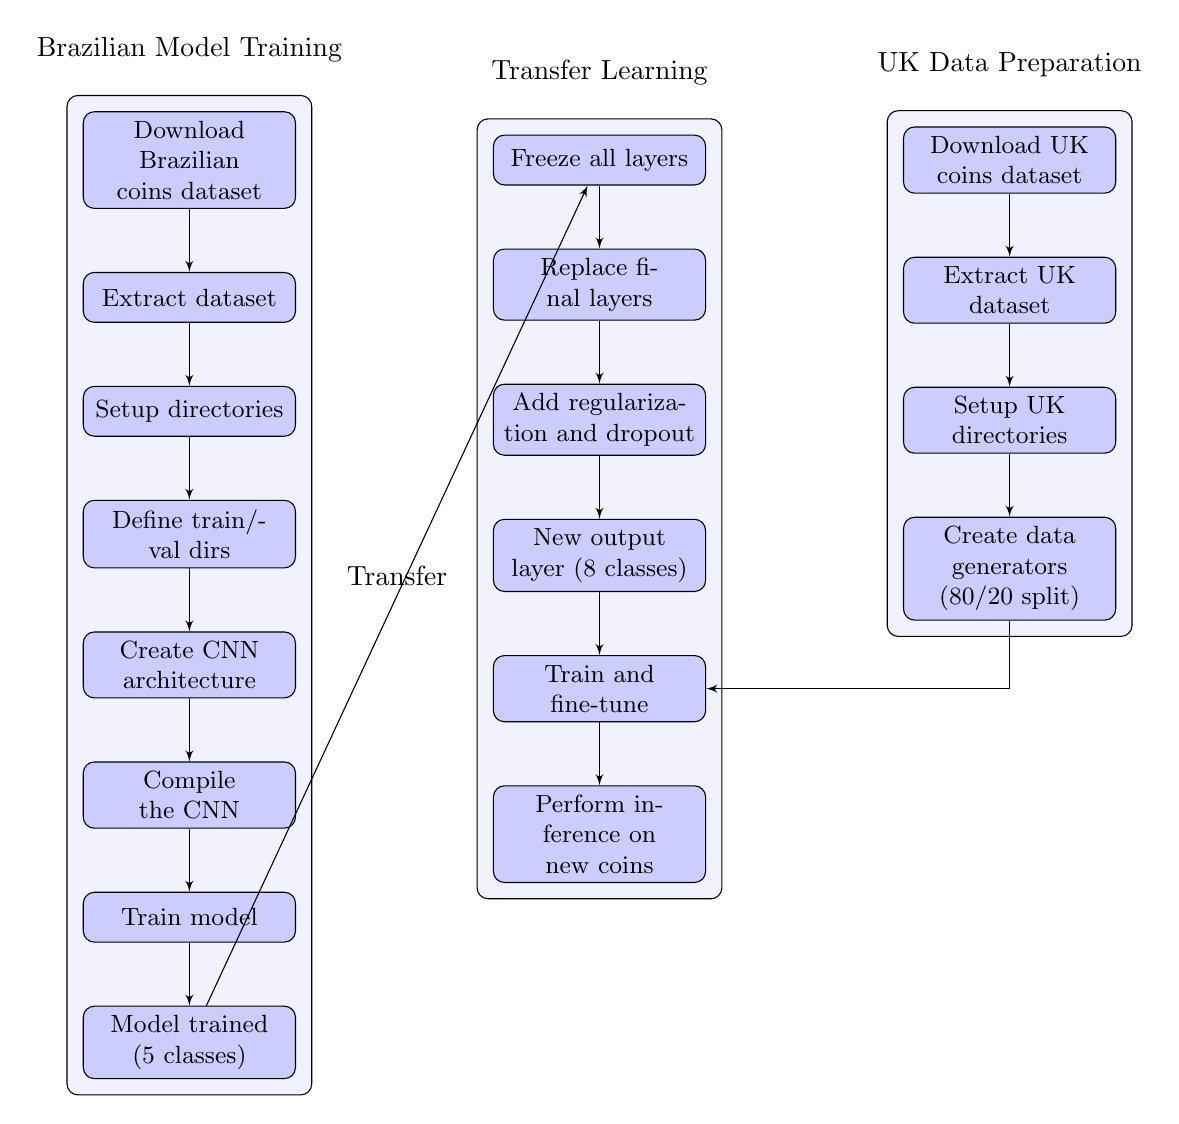
\begin{tikzpicture}[node distance=0.8cm and 1.5cm, auto]
    % Define a smaller block style
    \tikzset{
      block/.style = {rectangle, draw, fill=blue!20, 
                      text width=7em, text centered, rounded corners, minimum height=1.8em, font=\small},
    }
    
    % Brazilian model training - Column 1
    \node [block] (brazildata) {Download Brazilian coins dataset};
    \node [block, below=of brazildata] (extract) {Extract dataset};
    \node [block, below=of extract] (setup) {Setup directories};
    \node [block, below=of setup] (define) {Define train/val dirs};
    \node [block, below=of define] (create) {Create CNN architecture};
    \node [block, below=of create] (compile) {Compile the CNN};
    \node [block, below=of compile] (train) {Train model};
    \node [block, below=of train] (trained) {Model trained (5 classes)};
    
    % Transfer learning - Column 2 (Middle)
    \node [block, right=2.5cm of brazildata] (freeze) {Freeze all layers};
    \node [block, below=of freeze] (replace) {Replace final layers};
    \node [block, below=of replace] (add) {Add regularization and dropout};
    \node [block, below=of add] (output) {New output layer (8 classes)};
    \node [block, below=of output] (finaltrain) {Train and fine-tune};
    \node [block, below=of finaltrain] (inference) {Perform inference on new coins};
    
    % UK data preparation - Column 3 (Right)
    \node [block, right=2.5cm of freeze] (ukdata) {Download UK coins dataset};
    \node [block, below=of ukdata] (ukextract) {Extract UK dataset};
    \node [block, below=of ukextract] (uksetup) {Setup UK directories};
    \node [block, below=of uksetup] (ukgen) {Create data generators (80/20 split)};
    
    % Connect all nodes with arrows
    \path [line] (brazildata) -- (extract);
    \path [line] (extract) -- (setup);
    \path [line] (setup) -- (define);
    \path [line] (define) -- (create);
    \path [line] (create) -- (compile);
    \path [line] (compile) -- (train);
    \path [line] (train) -- (trained);
    
    \path [line] (ukdata) -- (ukextract);
    \path [line] (ukextract) -- (uksetup);
    \path [line] (uksetup) -- (ukgen);
    
    % Connect the columns
    \path [line] (trained) -- node[midway, above] {Transfer} (freeze);
    \path [line] (ukgen) |- (finaltrain);
    
    % Connect middle column
    \path [line] (freeze) -- (replace);
    \path [line] (replace) -- (add);
    \path [line] (add) -- (output);
    \path [line] (output) -- (finaltrain);
    \path [line] (finaltrain) -- (inference);
    
    % Group boxes to show different stages with smaller padding
    \begin{pgfonlayer}{background}
        \node[group={[yshift=0.3cm]above:Brazilian Model Training}, fit={(brazildata) (extract) (setup) (define) (create) (compile) (train) (trained)}, inner sep=0.2cm] {};
        \node[group={[yshift=0.3cm]above:UK Data Preparation}, fit={(ukdata) (ukextract) (uksetup) (ukgen)}, inner sep=0.2cm] {};
        \node[group={[yshift=0.3cm]above:Transfer Learning}, fit={(freeze) (replace) (add) (output) (finaltrain) (inference)}, inner sep=0.2cm] {};
    \end{pgfonlayer}
\end{tikzpicture}
}
% \caption{CNN Transfer Learning Flowchart: Brazilian to UK Coins}
% \label{fig:cnn-flowchart}
% \end{figure}
    }
    \caption{System Design Overview Flowchart}
    \label{fig:decriptiveLabel55} % descriptive to call in text with \ref{fig:decriptiveLabel55}
\end{figure}

\subsection{Functional Requirements}
% Your content here

\subsection{Design Approach}
% Your content here

\subsection{System Architecture}
As shown in Figure~\ref{fig:decriptiveLabel55} the system architecture consists of various components.

\begin{lstlisting}[style=cstyle, caption=System Architecture Code Example, label=lst:SystemArchitecture11]
# Your code here
\end{lstlisting}

\begin{figure}[htbp] %h-ere t-op b-ottom p-page (separte) -good to allow all htbp to give the compiler more options
    \centering
    \includegraphics[width=0.6\textwidth]{figures/methodology/system_architecture.jpg}
    \caption{System Architecture Diagram}
    \label{fig:system-architecture6}
\end{figure}
% SignalConditioningCircuitry.tex
% TestingApparatus.tex
\subsection{Signal Conditioning Circuitry} % \chapter{Methodology}>\section{Prototype}
\label{subsec:SignalConditioningCircuitry}

\paragraph{Photodiodes} produce a certain amount of current when light hits the depletion region. Therefore, a larger depletion region is desirable, to capture more light and in turn produce more current. For this purpose the photodiode in our circuit is reverse-biased as can be seen in Figure \ref{fig:AltiumDis} \cite[p.155]{RefWorks:keiser2021fiber}. 

%       ~~~   TIA SUB SUB SECTION   ~~~
%
\subsubsection{\acf{TIA}}
A reverse-biased photodiode allows a current to flow from the cathode to anode which is connected to ground. This current is converted to a Voltage using a \ac{TIA} with the following relationship derived as in Appendix Figure \ref{fig:Vo_deriv}:
\begin{equation} \label{eq:TIAoutput} % Voltage output TIA
  \begin{split}
  V_{\text{out}} = - I_{\text{ph}} \cdot R_f
  \end{split}
\end{equation}
\addequation{Transimpedance Amplifier Output Voltage}
\begin{equation} \label{eq:Photocurrent} % Current photodiode formula
  \begin{split}
  I_{\text{ph}} = P \cdot R_{\lambda}
  \end{split}
\end{equation}
\addequation{Photocurrent as Function of Optical Power}

Where $P$ is Light Power (W) and $R_{\lambda}$ is Responsivity (A/W).

\begin{equation} \label{eq:TIAoutputWithValues}
  \begin{split}
  V_{\text{out}} = -(P \cdot 0.5 \text{ A/W}) \cdot 1 \text{ M}\Omega
  \end{split}
\end{equation}
\addequation{TIA Output with Photodiode Response}

The \ac{TIA} circuit makes use of an \ac{OpAmp} as seen in Figure \ref{fig:AltiumDis} that provides very high imput impedance (1G$\Omega$) and allows the amplification of the signal without disturbing the photodiode current, therefore not affecting the readings. The inverting input is used in this configuration, which converts the negative current flowing from the cathode to the anode of the photodiode, into a positive voltage.

% Altium Diagram
%
\begin{figure}[htbp] %h-ere t-op b-ottom p-page (separte) -good to allow all htbp to give the compiler more options
    \centering
    \includegraphics[width=0.8\textwidth]{chapters/methodology/prototype/AltiumSingleCircuit_wCap.png}
    \caption{TIA and Post Amplification Circuit in Altium Designer}
    \label{fig:AltiumDis}
  \end{figure}
%
%       ~~~       SECONDARY AMPLIFICATION   ~~~
%
\subsubsection{Secondary Amplification}
\label{secondAmp}  
Testing showed that even using a 1M$\Omega$ resistor, the output voltage was too low (around 310mV) at our \ac{RED} testbench' \acp{LED} maximum brightness, as explained in Section \ref{explainPostAmp}. To raise the maximum Voltage to the desired maxium of the ADC of 5V, a higher feedback resistor could be used, however this would introduced noise and would require more complicated TIA with feedback capacitors. Due to the LM324-N having 4 \acp{OpAmp}, the decision was taken to implement a Secondary Amplification circuit. The non-inverting \ac{OpAmp} configuration was chosen to maintain the voltage positive, which also means there is no need for a dual power supply and keeps the Voltage positive for the Arduino ADC.
A simple calculation was made to figure out the required Gain of the circuit:
\begin{equation} \label{gainCalc}
  A = \frac{\text{required Voltage}}{\text{measured}} = \frac{5\text{ V}}{0.31\text{ V}} = 16.1
  \end{equation}
\addequation{Secondary Amplification Gain Calculation}

Knowing the gain required, the feedback resistor was calculated by choosing a 10k$\Omega R_1$ and rearranging the gain equation:

\begin{equation} \label{Feedback Resistor Calculation}
  \begin{split}
  A &= 1 + \frac{R_f}{R_1} \\
  16 &= 1 + \frac{R_f}{10\text{ k}\Omega} \\
  16 - 1 &= \frac{R_f}{10\text{ k}\Omega} \\
  15 &= \frac{R_f}{10\text{ k}\Omega} \\
  R_f &= 15 \times 10\text{ k}\Omega \\
  R_f &= 150\text{ k}\Omega
  \end{split}
\end{equation}
\addequation{Amplifier Feedback Resistor Calculation}

This provides a gain $A= 16$ which is very close to the Gain required in Equation \ref{gainCalc}. Further it must be stated that the resistors used have a tolerance of 10\% - therefore the actual final gain will fluctuate by that much. Once the design was tested on a BreadBoard, it was transfered to a stripboard as pictured in Figure \ref{fig:StripboardPhoto}.
Later in the design during testing, a decision was made to add a $1\mu$F capacitor in parallel with the feedback resistor of the Secondary Amplifier. This creates a low-pass filter on the output as seen in Eq. \ref{Low Pass Filter Calculation}.
\begin{equation} \label{Low Pass Filter Calculation}
  \begin{split}
    f_c &= \frac{1}{2\pi RC} \\
    f_c &= \frac{1}{2\pi \cdot 150\text{ k}\Omega \cdot 1\text{ }\mu\text{F}} \\
    f_c &= \frac{1}{2\pi \cdot 150 \cdot 10^3 \cdot 1 \cdot 10^{-6}\text{ s}} \\
    f_c &= \frac{1}{2\pi \cdot 150 \cdot 10^{-3}\text{ s}} \\
    f_c &= \frac{1}{0.942\text{ s}} \\
    f_c &= 1.061\text{ Hz}
  \end{split}
\end{equation}
\addequation{Secondary Amplification Low Pass Filter Calculation}

This does mean that we are now restricting the design to not be able to show Voltage change rates at higher than 1Hz, and testing with a moving light source will have to be restricted to a frequency at least half of 1Hz. Otherwise, the rate of change of Voltage will appear gradual and not represent the real signal. 

\begin{landscape}
  \includepdf[pages=1,angle=90]{chapters/methodology/prototype/altium_full.pdf}
\end{landscape}

%
% templates for figures, code, 
%

% %%% display code nicely
% \begin{lstlisting}[style=cstyle, caption=System Architecture Code Example, label=lst:SystemArchitecture7]
% # Your code here
% \end{lstlisting}

% \begin{figure}[htbp] %h-ere t-op b-ottom p-page (separte) -good to allow all htbp to give the compiler more options
%     \centering
%     \includegraphics[width=0.6\textwidth]{figures/methodology/system_architecture.jpg}
%     \caption{System Architecture Diagram}
%     \label{fig:system-architecture2}
% \end{figure}

% % Include a flowchart in LATEX format
% \begin{figure}[H]
%     \centering
%     \scalebox{0.8}{ % Scale to 80% of original size
%         % try generating flowcharts as svg in Claude 
% and edit with inkscape instead of this.
% but claude did generate this one so might 
% be useful too but you can't easily make
% small repairs in inkscape


% CNN Transfer Learning Flowchart - Compact Multi-Column Layout
% \begin{figure}[htbp]

\centering
\resizebox{\textwidth}{!}{ % Scale to fit width while maintaining aspect ratio
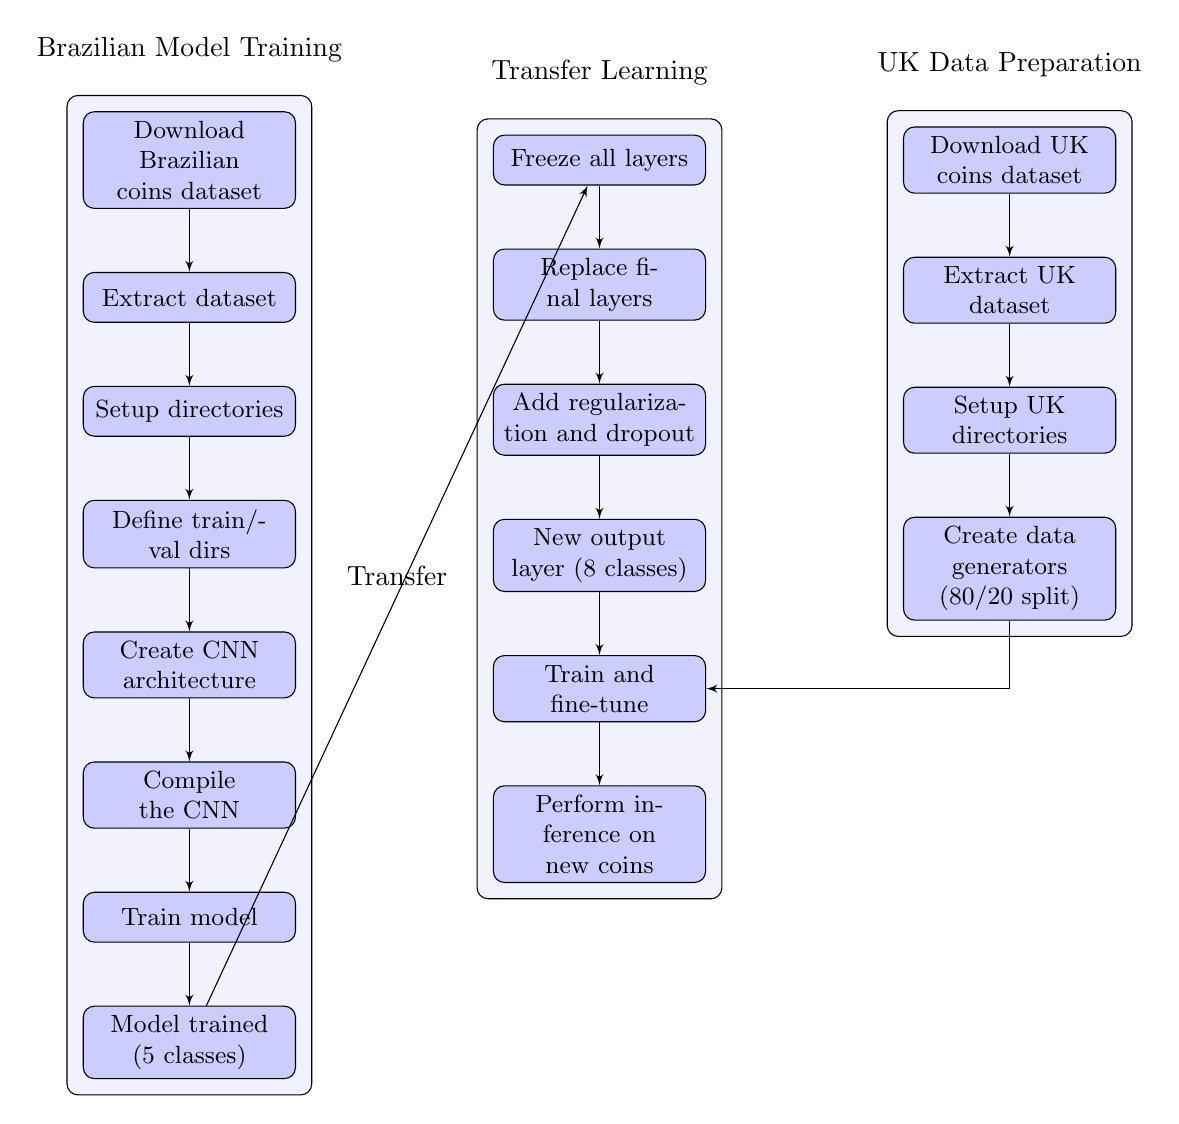
\begin{tikzpicture}[node distance=0.8cm and 1.5cm, auto]
    % Define a smaller block style
    \tikzset{
      block/.style = {rectangle, draw, fill=blue!20, 
                      text width=7em, text centered, rounded corners, minimum height=1.8em, font=\small},
    }
    
    % Brazilian model training - Column 1
    \node [block] (brazildata) {Download Brazilian coins dataset};
    \node [block, below=of brazildata] (extract) {Extract dataset};
    \node [block, below=of extract] (setup) {Setup directories};
    \node [block, below=of setup] (define) {Define train/val dirs};
    \node [block, below=of define] (create) {Create CNN architecture};
    \node [block, below=of create] (compile) {Compile the CNN};
    \node [block, below=of compile] (train) {Train model};
    \node [block, below=of train] (trained) {Model trained (5 classes)};
    
    % Transfer learning - Column 2 (Middle)
    \node [block, right=2.5cm of brazildata] (freeze) {Freeze all layers};
    \node [block, below=of freeze] (replace) {Replace final layers};
    \node [block, below=of replace] (add) {Add regularization and dropout};
    \node [block, below=of add] (output) {New output layer (8 classes)};
    \node [block, below=of output] (finaltrain) {Train and fine-tune};
    \node [block, below=of finaltrain] (inference) {Perform inference on new coins};
    
    % UK data preparation - Column 3 (Right)
    \node [block, right=2.5cm of freeze] (ukdata) {Download UK coins dataset};
    \node [block, below=of ukdata] (ukextract) {Extract UK dataset};
    \node [block, below=of ukextract] (uksetup) {Setup UK directories};
    \node [block, below=of uksetup] (ukgen) {Create data generators (80/20 split)};
    
    % Connect all nodes with arrows
    \path [line] (brazildata) -- (extract);
    \path [line] (extract) -- (setup);
    \path [line] (setup) -- (define);
    \path [line] (define) -- (create);
    \path [line] (create) -- (compile);
    \path [line] (compile) -- (train);
    \path [line] (train) -- (trained);
    
    \path [line] (ukdata) -- (ukextract);
    \path [line] (ukextract) -- (uksetup);
    \path [line] (uksetup) -- (ukgen);
    
    % Connect the columns
    \path [line] (trained) -- node[midway, above] {Transfer} (freeze);
    \path [line] (ukgen) |- (finaltrain);
    
    % Connect middle column
    \path [line] (freeze) -- (replace);
    \path [line] (replace) -- (add);
    \path [line] (add) -- (output);
    \path [line] (output) -- (finaltrain);
    \path [line] (finaltrain) -- (inference);
    
    % Group boxes to show different stages with smaller padding
    \begin{pgfonlayer}{background}
        \node[group={[yshift=0.3cm]above:Brazilian Model Training}, fit={(brazildata) (extract) (setup) (define) (create) (compile) (train) (trained)}, inner sep=0.2cm] {};
        \node[group={[yshift=0.3cm]above:UK Data Preparation}, fit={(ukdata) (ukextract) (uksetup) (ukgen)}, inner sep=0.2cm] {};
        \node[group={[yshift=0.3cm]above:Transfer Learning}, fit={(freeze) (replace) (add) (output) (finaltrain) (inference)}, inner sep=0.2cm] {};
    \end{pgfonlayer}
\end{tikzpicture}
}
% \caption{CNN Transfer Learning Flowchart: Brazilian to UK Coins}
% \label{fig:cnn-flowchart}
% \end{figure}
%     }
%     \caption{System Design Overview Flowchart}
%     \label{fig:decriptiveLabel11} % descriptive to call in text with \ref{fig:decriptiveLabel}
% \end{figure}
% EnclosureDesignAndFabrication.tex
\subsection{Enclosure Design 3D print}  % to adapt from Nass here? no need to follow titles below, 
\label{subsec:enclosureDesign}
                                        % but keep \subsubsection{} to maintain structure
                                        % \chapter{Methodology} > \section{Prototype} > \subsection{Enclosure..}
This section provides an overview on the design and fabrication of the enclosure for the prototype. The enclosure is a critical component that houses the electronic components and provides protection against environmental factors. The design process involves several steps, including conceptualization, modeling, and fabrication.


\subsubsection{Conceptualization}

\subsubsection{Material Selection}

\subsubsection{Fabrication Process}

\subsubsection{Testing and Validation}

\subsubsection{Iterations and Improvements}

\subsubsection{Final Enclousure Specifications and Documentation} 

%
% templates for figures, code, 
%

% %%% display code nicely
% \begin{lstlisting}[style=cstyle, caption=System Architecture Code Example, label=lst:SystemArchitecture7]
% # Your code here
% \end{lstlisting}

% \begin{figure}[htbp] %h-ere t-op b-ottom p-page (separte) -good to allow all htbp to give the compiler more options
%     \centering
%     \includegraphics[width=0.6\textwidth]{figures/methodology/system_architecture.jpg}
%     \caption{System Architecture Diagram}
%     \label{fig:system-architecture2}
% \end{figure}

% % Include a flowchart in LATEX format
% \begin{figure}[H]
%     \centering
%     \scalebox{0.8}{ % Scale to 80% of original size
%         % try generating flowcharts as svg in Claude 
% and edit with inkscape instead of this.
% but claude did generate this one so might 
% be useful too but you can't easily make
% small repairs in inkscape


% CNN Transfer Learning Flowchart - Compact Multi-Column Layout
% \begin{figure}[htbp]

\centering
\resizebox{\textwidth}{!}{ % Scale to fit width while maintaining aspect ratio
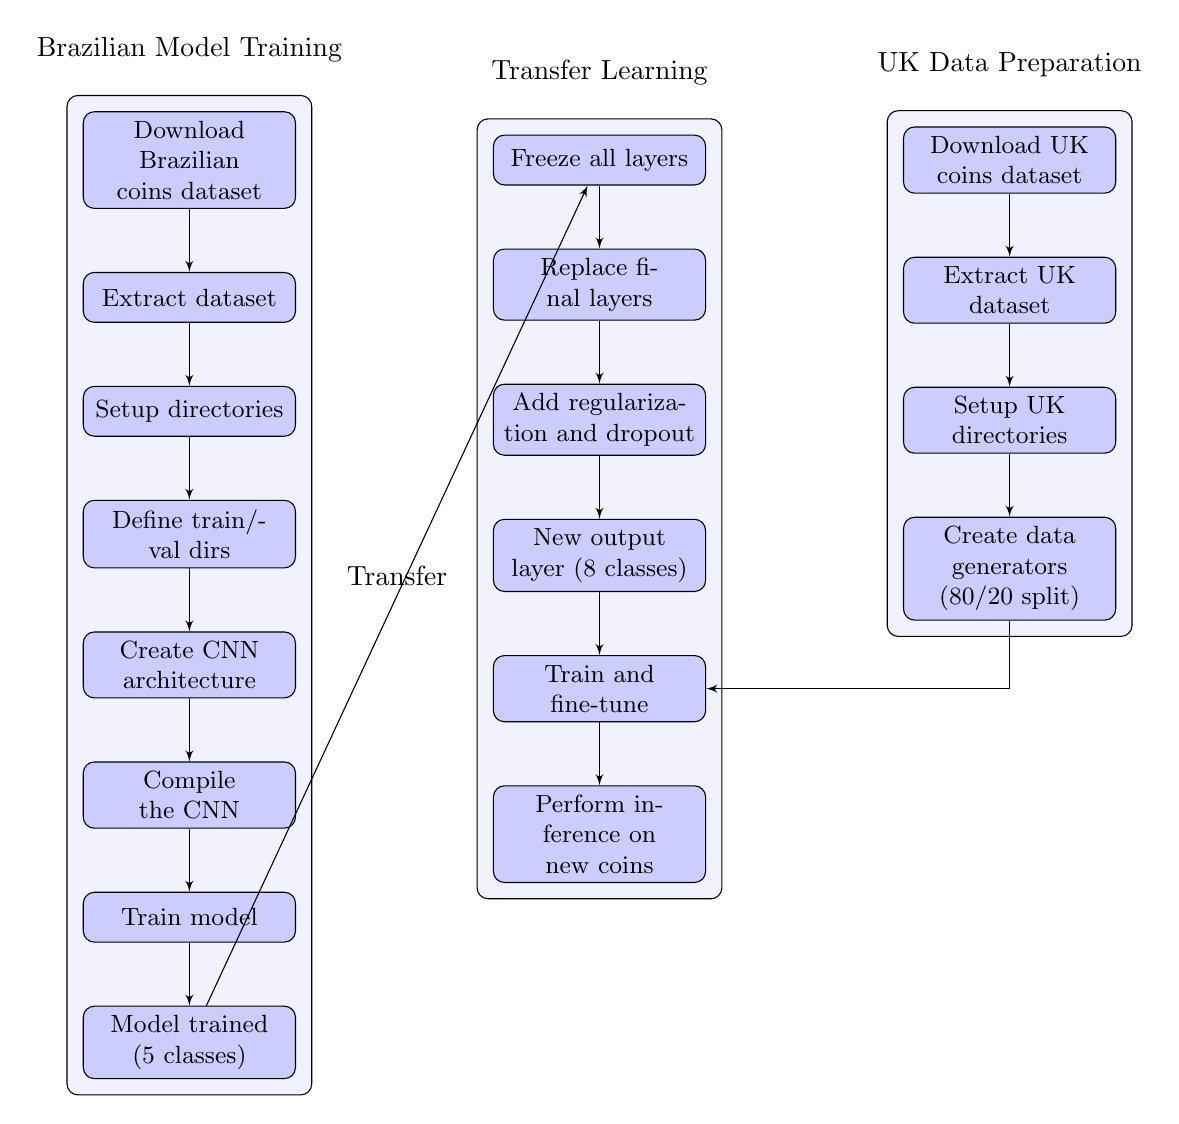
\begin{tikzpicture}[node distance=0.8cm and 1.5cm, auto]
    % Define a smaller block style
    \tikzset{
      block/.style = {rectangle, draw, fill=blue!20, 
                      text width=7em, text centered, rounded corners, minimum height=1.8em, font=\small},
    }
    
    % Brazilian model training - Column 1
    \node [block] (brazildata) {Download Brazilian coins dataset};
    \node [block, below=of brazildata] (extract) {Extract dataset};
    \node [block, below=of extract] (setup) {Setup directories};
    \node [block, below=of setup] (define) {Define train/val dirs};
    \node [block, below=of define] (create) {Create CNN architecture};
    \node [block, below=of create] (compile) {Compile the CNN};
    \node [block, below=of compile] (train) {Train model};
    \node [block, below=of train] (trained) {Model trained (5 classes)};
    
    % Transfer learning - Column 2 (Middle)
    \node [block, right=2.5cm of brazildata] (freeze) {Freeze all layers};
    \node [block, below=of freeze] (replace) {Replace final layers};
    \node [block, below=of replace] (add) {Add regularization and dropout};
    \node [block, below=of add] (output) {New output layer (8 classes)};
    \node [block, below=of output] (finaltrain) {Train and fine-tune};
    \node [block, below=of finaltrain] (inference) {Perform inference on new coins};
    
    % UK data preparation - Column 3 (Right)
    \node [block, right=2.5cm of freeze] (ukdata) {Download UK coins dataset};
    \node [block, below=of ukdata] (ukextract) {Extract UK dataset};
    \node [block, below=of ukextract] (uksetup) {Setup UK directories};
    \node [block, below=of uksetup] (ukgen) {Create data generators (80/20 split)};
    
    % Connect all nodes with arrows
    \path [line] (brazildata) -- (extract);
    \path [line] (extract) -- (setup);
    \path [line] (setup) -- (define);
    \path [line] (define) -- (create);
    \path [line] (create) -- (compile);
    \path [line] (compile) -- (train);
    \path [line] (train) -- (trained);
    
    \path [line] (ukdata) -- (ukextract);
    \path [line] (ukextract) -- (uksetup);
    \path [line] (uksetup) -- (ukgen);
    
    % Connect the columns
    \path [line] (trained) -- node[midway, above] {Transfer} (freeze);
    \path [line] (ukgen) |- (finaltrain);
    
    % Connect middle column
    \path [line] (freeze) -- (replace);
    \path [line] (replace) -- (add);
    \path [line] (add) -- (output);
    \path [line] (output) -- (finaltrain);
    \path [line] (finaltrain) -- (inference);
    
    % Group boxes to show different stages with smaller padding
    \begin{pgfonlayer}{background}
        \node[group={[yshift=0.3cm]above:Brazilian Model Training}, fit={(brazildata) (extract) (setup) (define) (create) (compile) (train) (trained)}, inner sep=0.2cm] {};
        \node[group={[yshift=0.3cm]above:UK Data Preparation}, fit={(ukdata) (ukextract) (uksetup) (ukgen)}, inner sep=0.2cm] {};
        \node[group={[yshift=0.3cm]above:Transfer Learning}, fit={(freeze) (replace) (add) (output) (finaltrain) (inference)}, inner sep=0.2cm] {};
    \end{pgfonlayer}
\end{tikzpicture}
}
% \caption{CNN Transfer Learning Flowchart: Brazilian to UK Coins}
% \label{fig:cnn-flowchart}
% \end{figure}
%     }
%     \caption{System Design Overview Flowchart}
%     \label{fig:decriptiveLabel11} % descriptive to call in text with \ref{fig:decriptiveLabel}
% \end{figure}
% DataAcquisitionSystem.tex
\section{Data Acquisition System}
This section provides an overview of the Data Acquisition System.

% Include a flowchart in TEX mode
\begin{figure}[H]
    \centering
    \scalebox{0.8}{ % Scale to 80% of original size
        % try generating flowcharts as svg in Claude 
% and edit with inkscape instead of this.
% but claude did generate this one so might 
% be useful too but you can't easily make
% small repairs in inkscape


% CNN Transfer Learning Flowchart - Compact Multi-Column Layout
% \begin{figure}[htbp]

\centering
\resizebox{\textwidth}{!}{ % Scale to fit width while maintaining aspect ratio
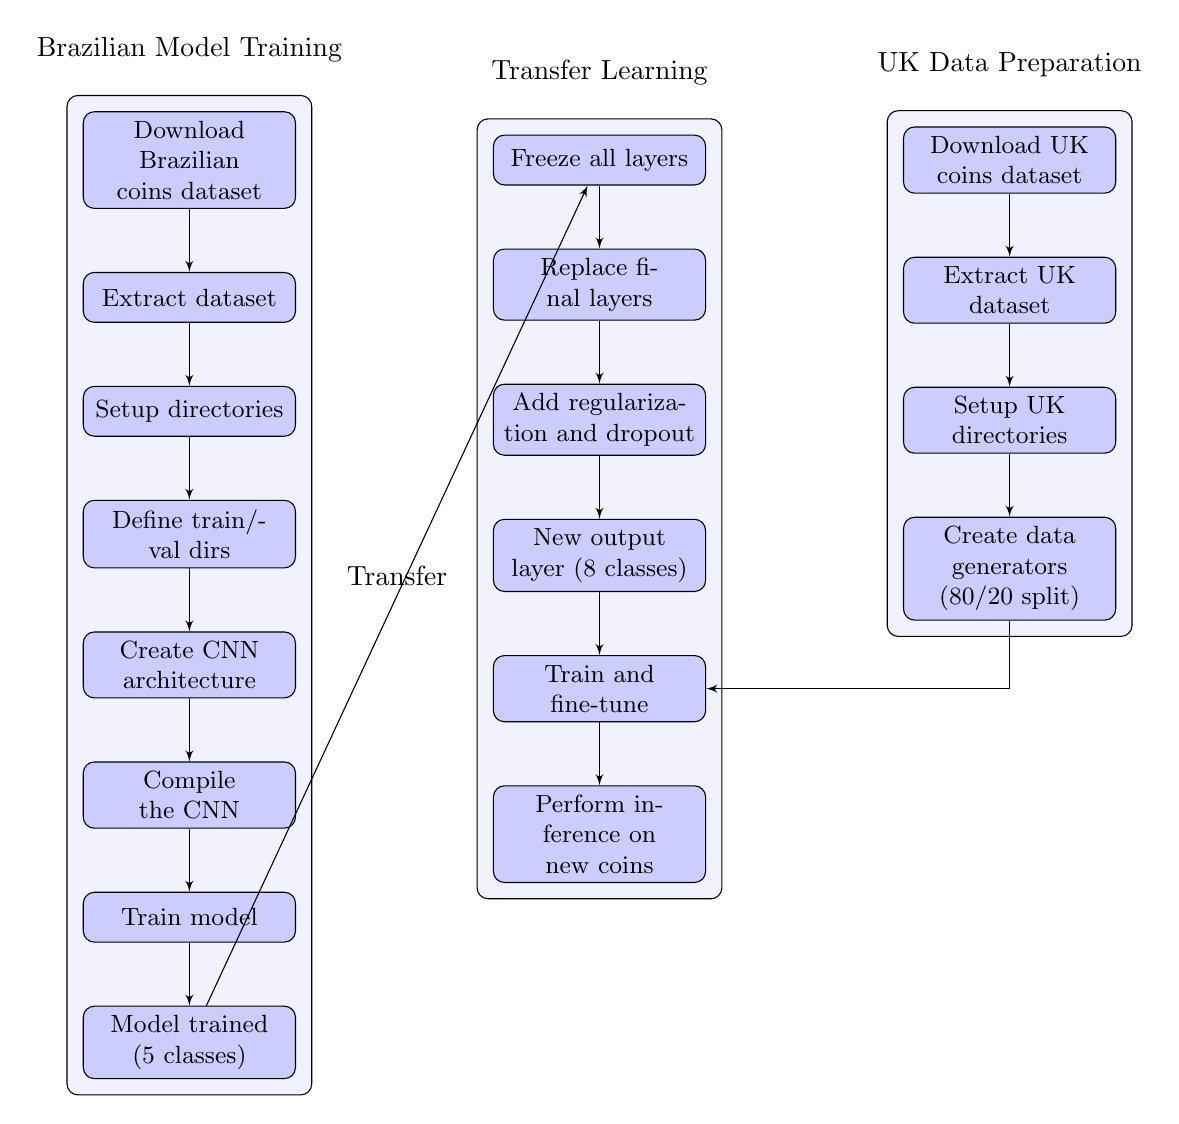
\begin{tikzpicture}[node distance=0.8cm and 1.5cm, auto]
    % Define a smaller block style
    \tikzset{
      block/.style = {rectangle, draw, fill=blue!20, 
                      text width=7em, text centered, rounded corners, minimum height=1.8em, font=\small},
    }
    
    % Brazilian model training - Column 1
    \node [block] (brazildata) {Download Brazilian coins dataset};
    \node [block, below=of brazildata] (extract) {Extract dataset};
    \node [block, below=of extract] (setup) {Setup directories};
    \node [block, below=of setup] (define) {Define train/val dirs};
    \node [block, below=of define] (create) {Create CNN architecture};
    \node [block, below=of create] (compile) {Compile the CNN};
    \node [block, below=of compile] (train) {Train model};
    \node [block, below=of train] (trained) {Model trained (5 classes)};
    
    % Transfer learning - Column 2 (Middle)
    \node [block, right=2.5cm of brazildata] (freeze) {Freeze all layers};
    \node [block, below=of freeze] (replace) {Replace final layers};
    \node [block, below=of replace] (add) {Add regularization and dropout};
    \node [block, below=of add] (output) {New output layer (8 classes)};
    \node [block, below=of output] (finaltrain) {Train and fine-tune};
    \node [block, below=of finaltrain] (inference) {Perform inference on new coins};
    
    % UK data preparation - Column 3 (Right)
    \node [block, right=2.5cm of freeze] (ukdata) {Download UK coins dataset};
    \node [block, below=of ukdata] (ukextract) {Extract UK dataset};
    \node [block, below=of ukextract] (uksetup) {Setup UK directories};
    \node [block, below=of uksetup] (ukgen) {Create data generators (80/20 split)};
    
    % Connect all nodes with arrows
    \path [line] (brazildata) -- (extract);
    \path [line] (extract) -- (setup);
    \path [line] (setup) -- (define);
    \path [line] (define) -- (create);
    \path [line] (create) -- (compile);
    \path [line] (compile) -- (train);
    \path [line] (train) -- (trained);
    
    \path [line] (ukdata) -- (ukextract);
    \path [line] (ukextract) -- (uksetup);
    \path [line] (uksetup) -- (ukgen);
    
    % Connect the columns
    \path [line] (trained) -- node[midway, above] {Transfer} (freeze);
    \path [line] (ukgen) |- (finaltrain);
    
    % Connect middle column
    \path [line] (freeze) -- (replace);
    \path [line] (replace) -- (add);
    \path [line] (add) -- (output);
    \path [line] (output) -- (finaltrain);
    \path [line] (finaltrain) -- (inference);
    
    % Group boxes to show different stages with smaller padding
    \begin{pgfonlayer}{background}
        \node[group={[yshift=0.3cm]above:Brazilian Model Training}, fit={(brazildata) (extract) (setup) (define) (create) (compile) (train) (trained)}, inner sep=0.2cm] {};
        \node[group={[yshift=0.3cm]above:UK Data Preparation}, fit={(ukdata) (ukextract) (uksetup) (ukgen)}, inner sep=0.2cm] {};
        \node[group={[yshift=0.3cm]above:Transfer Learning}, fit={(freeze) (replace) (add) (output) (finaltrain) (inference)}, inner sep=0.2cm] {};
    \end{pgfonlayer}
\end{tikzpicture}
}
% \caption{CNN Transfer Learning Flowchart: Brazilian to UK Coins}
% \label{fig:cnn-flowchart}
% \end{figure} % \input is for tex files \includegraphics is for images
    }
    \caption{System Design Overview Flowchart}
    \label{fig:decriptiveLabel22} % descriptive to call in text with \ref{fig:decriptiveLabel22}
\end{figure}


% other subsections
\subsection{Functional Requirements}
% Your content here

\subsection{Design Approach}
% Your content here

\subsection{System Architecture}
As shown in Figure~\ref{fig:decriptiveLabel22} the system architecture consists of various components.

\begin{lstlisting}[style=cstyle, caption=System Architecture Code Example, label=lst:SystemArchitecture8]
# Your code here
\end{lstlisting}

\begin{figure}[htbp] %h-ere t-op b-ottom p-page (separte) -good to allow all htbp to give the compiler more options
    \centering
    \includegraphics[width=0.6\textwidth]{figures/methodology/system_architecture.jpg}
    \caption{System Architecture Diagram}
    \label{fig:system-architecture3}
\end{figure}


\input{chapters/methodology/TestingApparatus}
% PrototypeDevelopmentLifecycle.tex
\section{Prototype Develop ment Lifecycle}
This section provides an overview of the Prototype Develop ment Lifecycle.

% Include a flowchart
\begin{figure}[H]
    \centering
    \scalebox{0.8}{ % Scale to 80% of original size
        % try generating flowcharts as svg in Claude 
% and edit with inkscape instead of this.
% but claude did generate this one so might 
% be useful too but you can't easily make
% small repairs in inkscape


% CNN Transfer Learning Flowchart - Compact Multi-Column Layout
% \begin{figure}[htbp]

\centering
\resizebox{\textwidth}{!}{ % Scale to fit width while maintaining aspect ratio
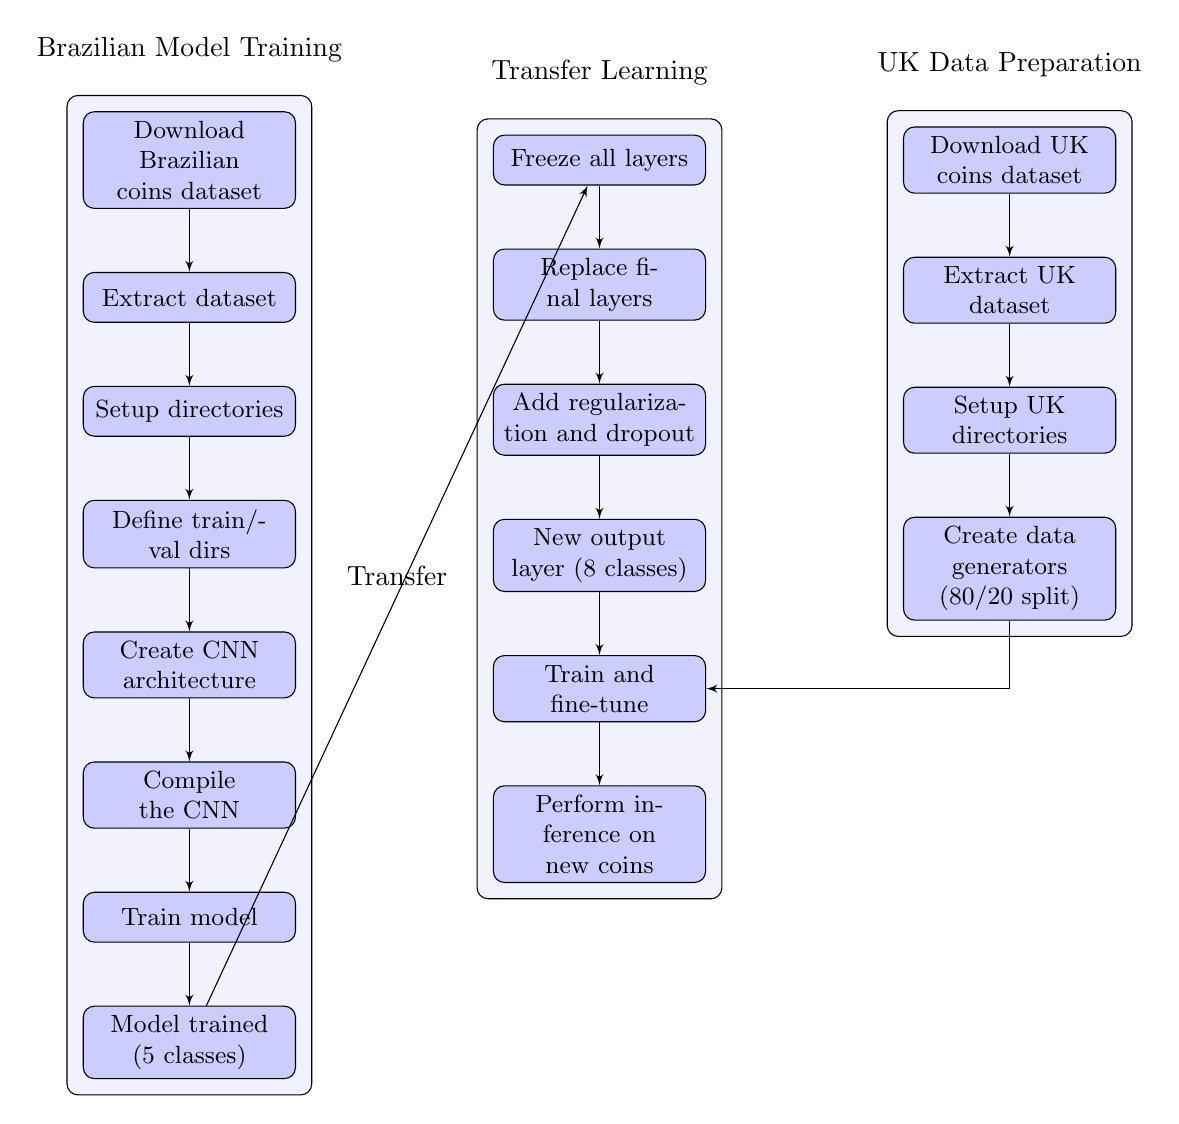
\begin{tikzpicture}[node distance=0.8cm and 1.5cm, auto]
    % Define a smaller block style
    \tikzset{
      block/.style = {rectangle, draw, fill=blue!20, 
                      text width=7em, text centered, rounded corners, minimum height=1.8em, font=\small},
    }
    
    % Brazilian model training - Column 1
    \node [block] (brazildata) {Download Brazilian coins dataset};
    \node [block, below=of brazildata] (extract) {Extract dataset};
    \node [block, below=of extract] (setup) {Setup directories};
    \node [block, below=of setup] (define) {Define train/val dirs};
    \node [block, below=of define] (create) {Create CNN architecture};
    \node [block, below=of create] (compile) {Compile the CNN};
    \node [block, below=of compile] (train) {Train model};
    \node [block, below=of train] (trained) {Model trained (5 classes)};
    
    % Transfer learning - Column 2 (Middle)
    \node [block, right=2.5cm of brazildata] (freeze) {Freeze all layers};
    \node [block, below=of freeze] (replace) {Replace final layers};
    \node [block, below=of replace] (add) {Add regularization and dropout};
    \node [block, below=of add] (output) {New output layer (8 classes)};
    \node [block, below=of output] (finaltrain) {Train and fine-tune};
    \node [block, below=of finaltrain] (inference) {Perform inference on new coins};
    
    % UK data preparation - Column 3 (Right)
    \node [block, right=2.5cm of freeze] (ukdata) {Download UK coins dataset};
    \node [block, below=of ukdata] (ukextract) {Extract UK dataset};
    \node [block, below=of ukextract] (uksetup) {Setup UK directories};
    \node [block, below=of uksetup] (ukgen) {Create data generators (80/20 split)};
    
    % Connect all nodes with arrows
    \path [line] (brazildata) -- (extract);
    \path [line] (extract) -- (setup);
    \path [line] (setup) -- (define);
    \path [line] (define) -- (create);
    \path [line] (create) -- (compile);
    \path [line] (compile) -- (train);
    \path [line] (train) -- (trained);
    
    \path [line] (ukdata) -- (ukextract);
    \path [line] (ukextract) -- (uksetup);
    \path [line] (uksetup) -- (ukgen);
    
    % Connect the columns
    \path [line] (trained) -- node[midway, above] {Transfer} (freeze);
    \path [line] (ukgen) |- (finaltrain);
    
    % Connect middle column
    \path [line] (freeze) -- (replace);
    \path [line] (replace) -- (add);
    \path [line] (add) -- (output);
    \path [line] (output) -- (finaltrain);
    \path [line] (finaltrain) -- (inference);
    
    % Group boxes to show different stages with smaller padding
    \begin{pgfonlayer}{background}
        \node[group={[yshift=0.3cm]above:Brazilian Model Training}, fit={(brazildata) (extract) (setup) (define) (create) (compile) (train) (trained)}, inner sep=0.2cm] {};
        \node[group={[yshift=0.3cm]above:UK Data Preparation}, fit={(ukdata) (ukextract) (uksetup) (ukgen)}, inner sep=0.2cm] {};
        \node[group={[yshift=0.3cm]above:Transfer Learning}, fit={(freeze) (replace) (add) (output) (finaltrain) (inference)}, inner sep=0.2cm] {};
    \end{pgfonlayer}
\end{tikzpicture}
}
% \caption{CNN Transfer Learning Flowchart: Brazilian to UK Coins}
% \label{fig:cnn-flowchart}
% \end{figure}
    }
    \caption{System Design Overview Flowchart}
    \label{fig:decriptiveLabel44} % descriptive to call in text with \ref{fig:decriptiveLabel44}
\end{figure}

\subsection{Functional Requirements}
% Your content here

\subsection{Design Approach}
% Your content here

\subsection{System Architecture}
As shown in Figure~\ref{fig:decriptiveLabel44} the system architecture consists of various components.

\begin{lstlisting}[style=cstyle, caption=System Architecture Code Example, label=lst:SystemArchitecture10]
# Your code here
\end{lstlisting}

\begin{figure}[htbp] %h-ere t-op b-ottom p-page (separte) -good to allow all htbp to give the compiler more options
    \centering
    \includegraphics[width=0.6\textwidth]{figures/methodology/system_architecture.jpg}
    \caption{System Architecture Diagram}
    \label{fig:system-architecture5}
\end{figure}

% test 
% Results.tex
\chapter{Results}

% Include each section from separate files
% SensorCharacterization.tex
\section{Sensor Characterization}
%
% THIS NEEDS CHANGING
%
%
TO FINISHTO FINISHTO FINISHTO FINISHTO FINISHTO FINISHTO FINISH focus on the fundamental properties and performance of your photodiodes themselves, distinct from the other subsections. Here are some key elements that would belong specifically under SensorCharacterization:

Basic Photodiode Electrical Characteristics:

Dark current measurements
Junction capacitance
I-V characteristics in different lighting conditions
Spectral response profiles (sensitivity vs. wavelength)


Individual Sensor Benchmarking:

Performance comparison between the 4 photodiodes (matching/differences)
Responsivity measurements (A/W)
Quantum efficiency calculations
Detection threshold levels

SNR!

Response Linearity:

Measurements showing linear range of the photodiodes
Saturation point characterization
Recovery time from saturation


Temperature Dependency:

Performance drift with temperature
Baseline shift measurements
Temperature compensation data


Aging/Stability Tests:

Long-term drift measurements
Repeatability of measurements over time



This section should focus on the inherent properties of the photodiodes themselves - essentially providing the baseline characterization data that underpins all the other analysis. The other sections then build on this foundation by examining how these sensors perform when integrated into the complete system with amplification, angular positioning, enclosure effects, etc.




% Example figure jpg
%
% \begin{figure}[htb]
%     \centering
%     \includegraphics[width=1\textwidth]{figures/results/system_architecture.jpg}
%     \caption{Overall System Performance Analysis}
%     \label{fig:systemPerformance}
% \end{figure}

% Example listing (such as text output from console)
% \begin{figure}[H]
%     \begin{lstlisting}[style=cstyle]
%     // Environmental test results
%     // Temperature, ambient light, and vibration effects
%     \end{lstlisting}
%     \caption{Environmental Testing Results}
%     \label{lst:EnvironmentalTests1}
%     \end{figure}



% LATEX flowchar
% Include a flowchart
% \begin{figure}[H]
%     \centering
%     \scalebox{0.8}{ % Scale to 80% of original size
%         % try generating flowcharts as svg in Claude 
% and edit with inkscape instead of this.
% but claude did generate this one so might 
% be useful too but you can't easily make
% small repairs in inkscape


% CNN Transfer Learning Flowchart - Compact Multi-Column Layout
% \begin{figure}[htbp]

\centering
\resizebox{\textwidth}{!}{ % Scale to fit width while maintaining aspect ratio
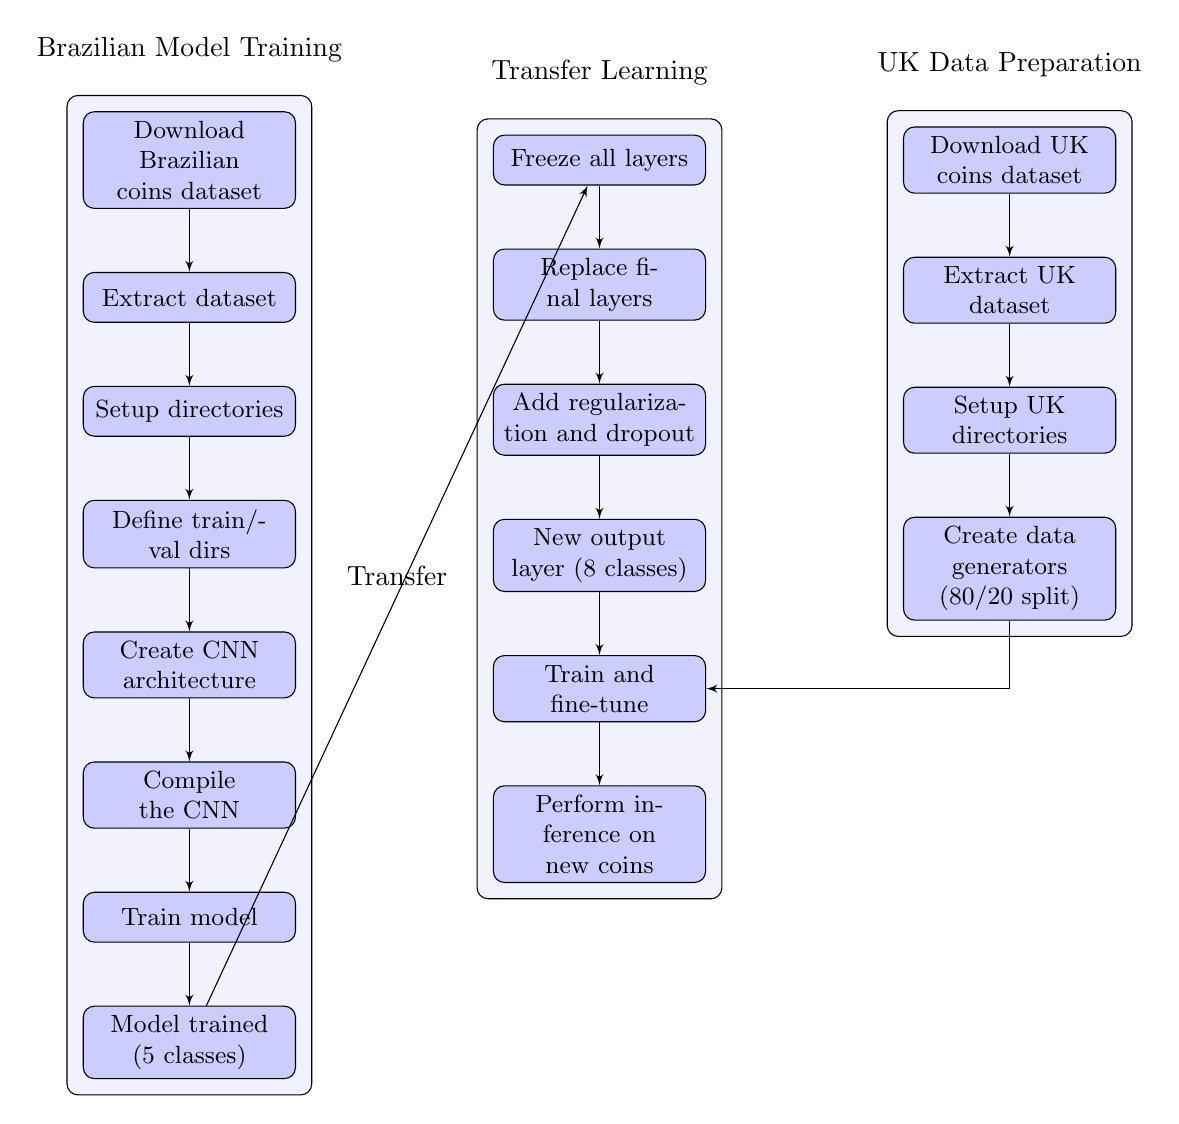
\begin{tikzpicture}[node distance=0.8cm and 1.5cm, auto]
    % Define a smaller block style
    \tikzset{
      block/.style = {rectangle, draw, fill=blue!20, 
                      text width=7em, text centered, rounded corners, minimum height=1.8em, font=\small},
    }
    
    % Brazilian model training - Column 1
    \node [block] (brazildata) {Download Brazilian coins dataset};
    \node [block, below=of brazildata] (extract) {Extract dataset};
    \node [block, below=of extract] (setup) {Setup directories};
    \node [block, below=of setup] (define) {Define train/val dirs};
    \node [block, below=of define] (create) {Create CNN architecture};
    \node [block, below=of create] (compile) {Compile the CNN};
    \node [block, below=of compile] (train) {Train model};
    \node [block, below=of train] (trained) {Model trained (5 classes)};
    
    % Transfer learning - Column 2 (Middle)
    \node [block, right=2.5cm of brazildata] (freeze) {Freeze all layers};
    \node [block, below=of freeze] (replace) {Replace final layers};
    \node [block, below=of replace] (add) {Add regularization and dropout};
    \node [block, below=of add] (output) {New output layer (8 classes)};
    \node [block, below=of output] (finaltrain) {Train and fine-tune};
    \node [block, below=of finaltrain] (inference) {Perform inference on new coins};
    
    % UK data preparation - Column 3 (Right)
    \node [block, right=2.5cm of freeze] (ukdata) {Download UK coins dataset};
    \node [block, below=of ukdata] (ukextract) {Extract UK dataset};
    \node [block, below=of ukextract] (uksetup) {Setup UK directories};
    \node [block, below=of uksetup] (ukgen) {Create data generators (80/20 split)};
    
    % Connect all nodes with arrows
    \path [line] (brazildata) -- (extract);
    \path [line] (extract) -- (setup);
    \path [line] (setup) -- (define);
    \path [line] (define) -- (create);
    \path [line] (create) -- (compile);
    \path [line] (compile) -- (train);
    \path [line] (train) -- (trained);
    
    \path [line] (ukdata) -- (ukextract);
    \path [line] (ukextract) -- (uksetup);
    \path [line] (uksetup) -- (ukgen);
    
    % Connect the columns
    \path [line] (trained) -- node[midway, above] {Transfer} (freeze);
    \path [line] (ukgen) |- (finaltrain);
    
    % Connect middle column
    \path [line] (freeze) -- (replace);
    \path [line] (replace) -- (add);
    \path [line] (add) -- (output);
    \path [line] (output) -- (finaltrain);
    \path [line] (finaltrain) -- (inference);
    
    % Group boxes to show different stages with smaller padding
    \begin{pgfonlayer}{background}
        \node[group={[yshift=0.3cm]above:Brazilian Model Training}, fit={(brazildata) (extract) (setup) (define) (create) (compile) (train) (trained)}, inner sep=0.2cm] {};
        \node[group={[yshift=0.3cm]above:UK Data Preparation}, fit={(ukdata) (ukextract) (uksetup) (ukgen)}, inner sep=0.2cm] {};
        \node[group={[yshift=0.3cm]above:Transfer Learning}, fit={(freeze) (replace) (add) (output) (finaltrain) (inference)}, inner sep=0.2cm] {};
    \end{pgfonlayer}
\end{tikzpicture}
}
% \caption{CNN Transfer Learning Flowchart: Brazilian to UK Coins}
% \label{fig:cnn-flowchart}
% \end{figure}
%     }
%     \caption{System Design Overview Flowchart}
%     \label{fig:decriptiveLabel3} % descriptive to call in text with \ref{fig:decriptiveLabel}
% \end{figure}

% AmplificationPerformance.tex
\section{Amplification Performance}
This section provides results of the amplifier performance.

% Include a flowchart
\begin{figure}[H]
    \centering
    \scalebox{0.5}{ % Scale to 80% of original size
        % try generating flowcharts as svg in Claude 
% and edit with inkscape instead of this.
% but claude did generate this one so might 
% be useful too but you can't easily make
% small repairs in inkscape


% CNN Transfer Learning Flowchart - Compact Multi-Column Layout
% \begin{figure}[htbp]

\centering
\resizebox{\textwidth}{!}{ % Scale to fit width while maintaining aspect ratio
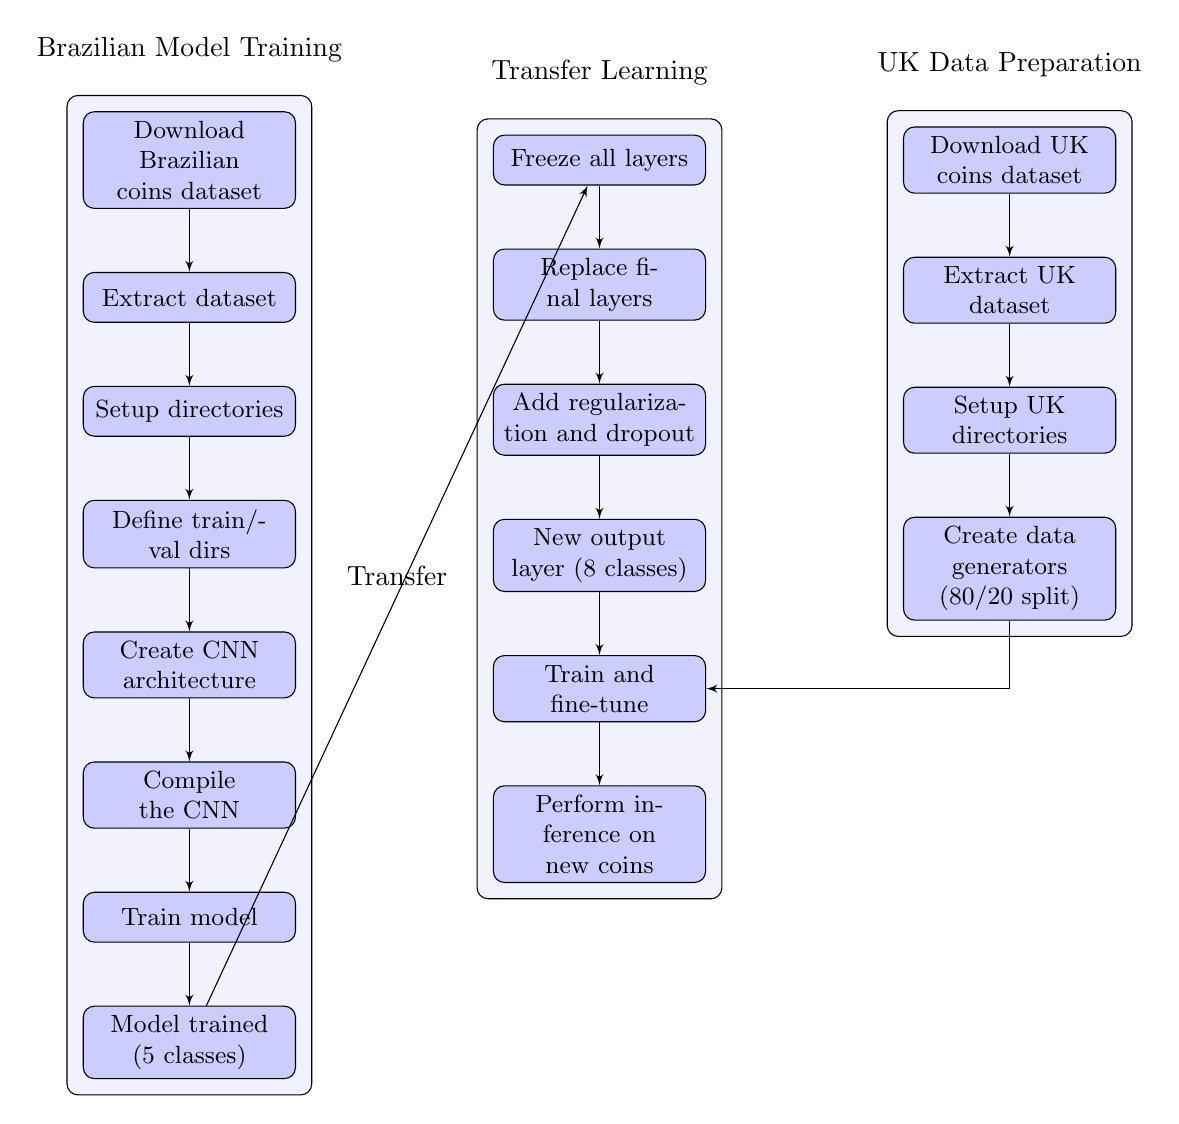
\begin{tikzpicture}[node distance=0.8cm and 1.5cm, auto]
    % Define a smaller block style
    \tikzset{
      block/.style = {rectangle, draw, fill=blue!20, 
                      text width=7em, text centered, rounded corners, minimum height=1.8em, font=\small},
    }
    
    % Brazilian model training - Column 1
    \node [block] (brazildata) {Download Brazilian coins dataset};
    \node [block, below=of brazildata] (extract) {Extract dataset};
    \node [block, below=of extract] (setup) {Setup directories};
    \node [block, below=of setup] (define) {Define train/val dirs};
    \node [block, below=of define] (create) {Create CNN architecture};
    \node [block, below=of create] (compile) {Compile the CNN};
    \node [block, below=of compile] (train) {Train model};
    \node [block, below=of train] (trained) {Model trained (5 classes)};
    
    % Transfer learning - Column 2 (Middle)
    \node [block, right=2.5cm of brazildata] (freeze) {Freeze all layers};
    \node [block, below=of freeze] (replace) {Replace final layers};
    \node [block, below=of replace] (add) {Add regularization and dropout};
    \node [block, below=of add] (output) {New output layer (8 classes)};
    \node [block, below=of output] (finaltrain) {Train and fine-tune};
    \node [block, below=of finaltrain] (inference) {Perform inference on new coins};
    
    % UK data preparation - Column 3 (Right)
    \node [block, right=2.5cm of freeze] (ukdata) {Download UK coins dataset};
    \node [block, below=of ukdata] (ukextract) {Extract UK dataset};
    \node [block, below=of ukextract] (uksetup) {Setup UK directories};
    \node [block, below=of uksetup] (ukgen) {Create data generators (80/20 split)};
    
    % Connect all nodes with arrows
    \path [line] (brazildata) -- (extract);
    \path [line] (extract) -- (setup);
    \path [line] (setup) -- (define);
    \path [line] (define) -- (create);
    \path [line] (create) -- (compile);
    \path [line] (compile) -- (train);
    \path [line] (train) -- (trained);
    
    \path [line] (ukdata) -- (ukextract);
    \path [line] (ukextract) -- (uksetup);
    \path [line] (uksetup) -- (ukgen);
    
    % Connect the columns
    \path [line] (trained) -- node[midway, above] {Transfer} (freeze);
    \path [line] (ukgen) |- (finaltrain);
    
    % Connect middle column
    \path [line] (freeze) -- (replace);
    \path [line] (replace) -- (add);
    \path [line] (add) -- (output);
    \path [line] (output) -- (finaltrain);
    \path [line] (finaltrain) -- (inference);
    
    % Group boxes to show different stages with smaller padding
    \begin{pgfonlayer}{background}
        \node[group={[yshift=0.3cm]above:Brazilian Model Training}, fit={(brazildata) (extract) (setup) (define) (create) (compile) (train) (trained)}, inner sep=0.2cm] {};
        \node[group={[yshift=0.3cm]above:UK Data Preparation}, fit={(ukdata) (ukextract) (uksetup) (ukgen)}, inner sep=0.2cm] {};
        \node[group={[yshift=0.3cm]above:Transfer Learning}, fit={(freeze) (replace) (add) (output) (finaltrain) (inference)}, inner sep=0.2cm] {};
    \end{pgfonlayer}
\end{tikzpicture}
}
% \caption{CNN Transfer Learning Flowchart: Brazilian to UK Coins}
% \label{fig:cnn-flowchart}
% \end{figure}
    }
    \caption{System Design Overview Flowchart}
    \label{fig:decriptiveLabel1} % descriptive to call in text with \ref{fig:decriptiveLabel}
\end{figure}

\subsection{Functional Requirements}
% Your content here

\subsection{Design Approach}
% Your content here

\subsection{System Architecture}
As shown in Figure~\ref{fig:decriptiveLabel1} the system architecture consists of various components.

\begin{lstlisting}[style=cstyle, caption=System Architecture Code Example, label=lst:SystemArchitecture6]
# Your code here
\end{lstlisting}

\begin{figure}[htbp] %h-ere t-op b-ottom p-page (separte) -good to allow all htbp to give the compiler more options
    \centering
    \includegraphics[width=0.6\textwidth]{figures/results/system_architecture.jpg}
    \caption{System Architecture Diagram}
    \label{fig:system-architecture20}
\end{figure}
% PhotodiodeAngularResponse.tex
\section{Photodiode Angular Response}
This section discusses the results of the response of the solar sensor to angular changes of the light source.








% Example figure jpg
%
% \begin{figure}[htb]
%     \centering
%     \includegraphics[width=1\textwidth]{figures/results/system_architecture.jpg}
%     \caption{Overall System Performance Analysis}
%     \label{fig:systemPerformance}
% \end{figure}

% Example listing (such as text output from console)
% \begin{figure}[H]
%     \begin{lstlisting}[style=cstyle]
%     // Environmental test results
%     // Temperature, ambient light, and vibration effects
%     \end{lstlisting}
%     \caption{Environmental Testing Results}
%     \label{lst:EnvironmentalTests1}
%     \end{figure}



% LATEX flowchar
% Include a flowchart
% \begin{figure}[H]
%     \centering
%     \scalebox{0.8}{ % Scale to 80% of original size
%         % try generating flowcharts as svg in Claude 
% and edit with inkscape instead of this.
% but claude did generate this one so might 
% be useful too but you can't easily make
% small repairs in inkscape


% CNN Transfer Learning Flowchart - Compact Multi-Column Layout
% \begin{figure}[htbp]

\centering
\resizebox{\textwidth}{!}{ % Scale to fit width while maintaining aspect ratio
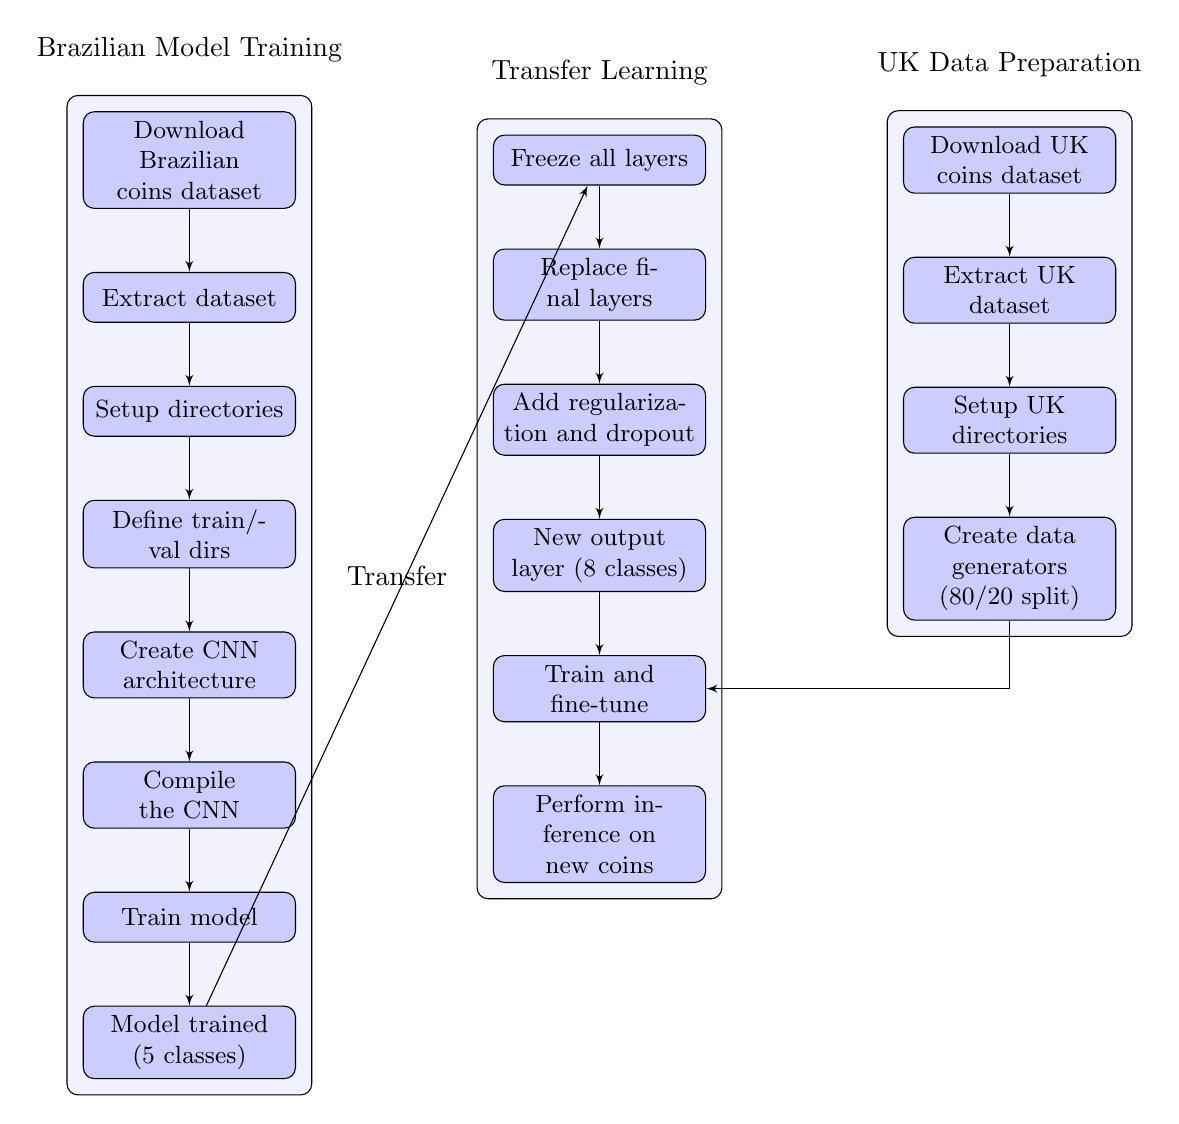
\begin{tikzpicture}[node distance=0.8cm and 1.5cm, auto]
    % Define a smaller block style
    \tikzset{
      block/.style = {rectangle, draw, fill=blue!20, 
                      text width=7em, text centered, rounded corners, minimum height=1.8em, font=\small},
    }
    
    % Brazilian model training - Column 1
    \node [block] (brazildata) {Download Brazilian coins dataset};
    \node [block, below=of brazildata] (extract) {Extract dataset};
    \node [block, below=of extract] (setup) {Setup directories};
    \node [block, below=of setup] (define) {Define train/val dirs};
    \node [block, below=of define] (create) {Create CNN architecture};
    \node [block, below=of create] (compile) {Compile the CNN};
    \node [block, below=of compile] (train) {Train model};
    \node [block, below=of train] (trained) {Model trained (5 classes)};
    
    % Transfer learning - Column 2 (Middle)
    \node [block, right=2.5cm of brazildata] (freeze) {Freeze all layers};
    \node [block, below=of freeze] (replace) {Replace final layers};
    \node [block, below=of replace] (add) {Add regularization and dropout};
    \node [block, below=of add] (output) {New output layer (8 classes)};
    \node [block, below=of output] (finaltrain) {Train and fine-tune};
    \node [block, below=of finaltrain] (inference) {Perform inference on new coins};
    
    % UK data preparation - Column 3 (Right)
    \node [block, right=2.5cm of freeze] (ukdata) {Download UK coins dataset};
    \node [block, below=of ukdata] (ukextract) {Extract UK dataset};
    \node [block, below=of ukextract] (uksetup) {Setup UK directories};
    \node [block, below=of uksetup] (ukgen) {Create data generators (80/20 split)};
    
    % Connect all nodes with arrows
    \path [line] (brazildata) -- (extract);
    \path [line] (extract) -- (setup);
    \path [line] (setup) -- (define);
    \path [line] (define) -- (create);
    \path [line] (create) -- (compile);
    \path [line] (compile) -- (train);
    \path [line] (train) -- (trained);
    
    \path [line] (ukdata) -- (ukextract);
    \path [line] (ukextract) -- (uksetup);
    \path [line] (uksetup) -- (ukgen);
    
    % Connect the columns
    \path [line] (trained) -- node[midway, above] {Transfer} (freeze);
    \path [line] (ukgen) |- (finaltrain);
    
    % Connect middle column
    \path [line] (freeze) -- (replace);
    \path [line] (replace) -- (add);
    \path [line] (add) -- (output);
    \path [line] (output) -- (finaltrain);
    \path [line] (finaltrain) -- (inference);
    
    % Group boxes to show different stages with smaller padding
    \begin{pgfonlayer}{background}
        \node[group={[yshift=0.3cm]above:Brazilian Model Training}, fit={(brazildata) (extract) (setup) (define) (create) (compile) (train) (trained)}, inner sep=0.2cm] {};
        \node[group={[yshift=0.3cm]above:UK Data Preparation}, fit={(ukdata) (ukextract) (uksetup) (ukgen)}, inner sep=0.2cm] {};
        \node[group={[yshift=0.3cm]above:Transfer Learning}, fit={(freeze) (replace) (add) (output) (finaltrain) (inference)}, inner sep=0.2cm] {};
    \end{pgfonlayer}
\end{tikzpicture}
}
% \caption{CNN Transfer Learning Flowchart: Brazilian to UK Coins}
% \label{fig:cnn-flowchart}
% \end{figure}
%     }
%     \caption{System Design Overview Flowchart}
%     \label{fig:decriptiveLabel3} % descriptive to call in text with \ref{fig:decriptiveLabel}
% \end{figure}
% EnclosureEffectiveness.tex
\section{Enclosure Effectiveness}
This section discusses the effectiveness of the Photodiode enlosure.

% % Include a flowchart
% \begin{figure}[H]
%     \centering
%     \scalebox{0.8}{ % Scale to 80% of original size
%         % try generating flowcharts as svg in Claude 
% and edit with inkscape instead of this.
% but claude did generate this one so might 
% be useful too but you can't easily make
% small repairs in inkscape


% CNN Transfer Learning Flowchart - Compact Multi-Column Layout
% \begin{figure}[htbp]

\centering
\resizebox{\textwidth}{!}{ % Scale to fit width while maintaining aspect ratio
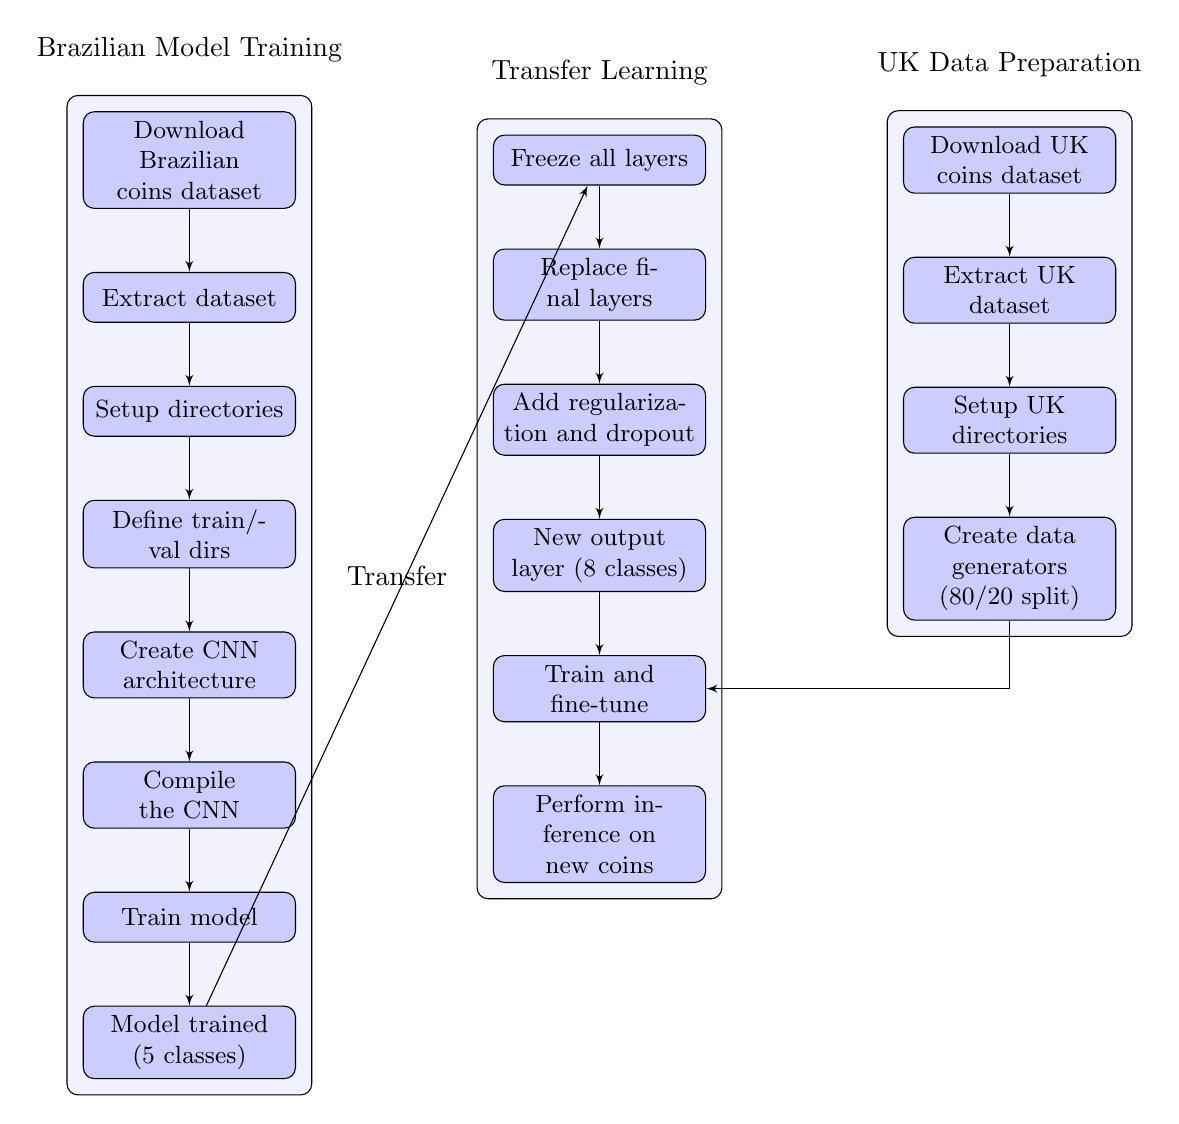
\begin{tikzpicture}[node distance=0.8cm and 1.5cm, auto]
    % Define a smaller block style
    \tikzset{
      block/.style = {rectangle, draw, fill=blue!20, 
                      text width=7em, text centered, rounded corners, minimum height=1.8em, font=\small},
    }
    
    % Brazilian model training - Column 1
    \node [block] (brazildata) {Download Brazilian coins dataset};
    \node [block, below=of brazildata] (extract) {Extract dataset};
    \node [block, below=of extract] (setup) {Setup directories};
    \node [block, below=of setup] (define) {Define train/val dirs};
    \node [block, below=of define] (create) {Create CNN architecture};
    \node [block, below=of create] (compile) {Compile the CNN};
    \node [block, below=of compile] (train) {Train model};
    \node [block, below=of train] (trained) {Model trained (5 classes)};
    
    % Transfer learning - Column 2 (Middle)
    \node [block, right=2.5cm of brazildata] (freeze) {Freeze all layers};
    \node [block, below=of freeze] (replace) {Replace final layers};
    \node [block, below=of replace] (add) {Add regularization and dropout};
    \node [block, below=of add] (output) {New output layer (8 classes)};
    \node [block, below=of output] (finaltrain) {Train and fine-tune};
    \node [block, below=of finaltrain] (inference) {Perform inference on new coins};
    
    % UK data preparation - Column 3 (Right)
    \node [block, right=2.5cm of freeze] (ukdata) {Download UK coins dataset};
    \node [block, below=of ukdata] (ukextract) {Extract UK dataset};
    \node [block, below=of ukextract] (uksetup) {Setup UK directories};
    \node [block, below=of uksetup] (ukgen) {Create data generators (80/20 split)};
    
    % Connect all nodes with arrows
    \path [line] (brazildata) -- (extract);
    \path [line] (extract) -- (setup);
    \path [line] (setup) -- (define);
    \path [line] (define) -- (create);
    \path [line] (create) -- (compile);
    \path [line] (compile) -- (train);
    \path [line] (train) -- (trained);
    
    \path [line] (ukdata) -- (ukextract);
    \path [line] (ukextract) -- (uksetup);
    \path [line] (uksetup) -- (ukgen);
    
    % Connect the columns
    \path [line] (trained) -- node[midway, above] {Transfer} (freeze);
    \path [line] (ukgen) |- (finaltrain);
    
    % Connect middle column
    \path [line] (freeze) -- (replace);
    \path [line] (replace) -- (add);
    \path [line] (add) -- (output);
    \path [line] (output) -- (finaltrain);
    \path [line] (finaltrain) -- (inference);
    
    % Group boxes to show different stages with smaller padding
    \begin{pgfonlayer}{background}
        \node[group={[yshift=0.3cm]above:Brazilian Model Training}, fit={(brazildata) (extract) (setup) (define) (create) (compile) (train) (trained)}, inner sep=0.2cm] {};
        \node[group={[yshift=0.3cm]above:UK Data Preparation}, fit={(ukdata) (ukextract) (uksetup) (ukgen)}, inner sep=0.2cm] {};
        \node[group={[yshift=0.3cm]above:Transfer Learning}, fit={(freeze) (replace) (add) (output) (finaltrain) (inference)}, inner sep=0.2cm] {};
    \end{pgfonlayer}
\end{tikzpicture}
}
% \caption{CNN Transfer Learning Flowchart: Brazilian to UK Coins}
% \label{fig:cnn-flowchart}
% \end{figure}
%     }
%     \caption{System Design Overview Flowchart}
%     \label{fig:decriptiveLabel5} % descriptive to call in text with \ref{fig:decriptiveLabel}
% \end{figure}

% \subsection{Functional Requirements}
% % Your content here

% \subsection{Design Approach}
% % Your content here

% \subsection{System Architecture}
% As shown in Figure~\ref{fig:decriptiveLabel5} the system architecture consists of various components.

% \begin{lstlisting}[style=cstyle, caption=System Architecture Code Example, label=lst:SystemArchitecture4]
% # Your code here
% \end{lstlisting}

% \begin{figure}[htbp] %h-ere t-op b-ottom p-page (separte) -good to allow all htbp to give the compiler more options
%     \centering
%     \includegraphics[width=0.6\textwidth]{figures/results/system_architecture.jpg}
%     \caption{System Architecture Diagram}
%     \label{fig:system-architecture22}
% \end{figure}
% DataAcquisitionSystemEvaluation.tex
\section{\acf{DAQ} System Evaluation}
The \ac{DAQ} was considered a success, it was able to take recordings in realtime of all four photodiodes and send them to a computer for post-processing. In it's final design the overal system that included the Python script as well as the Arduino, was able to perform it's task of generating both data in csv format that allowed comparison with simulated input, as well as the addition of noise filtering. % maybe add \ref to figures with graph 

% % Include a flowchart
% \begin{figure}[H]
%     \centering
%     \scalebox{0.8}{ % Scale to 80% of original size
%         % try generating flowcharts as svg in Claude 
% and edit with inkscape instead of this.
% but claude did generate this one so might 
% be useful too but you can't easily make
% small repairs in inkscape


% CNN Transfer Learning Flowchart - Compact Multi-Column Layout
% \begin{figure}[htbp]

\centering
\resizebox{\textwidth}{!}{ % Scale to fit width while maintaining aspect ratio
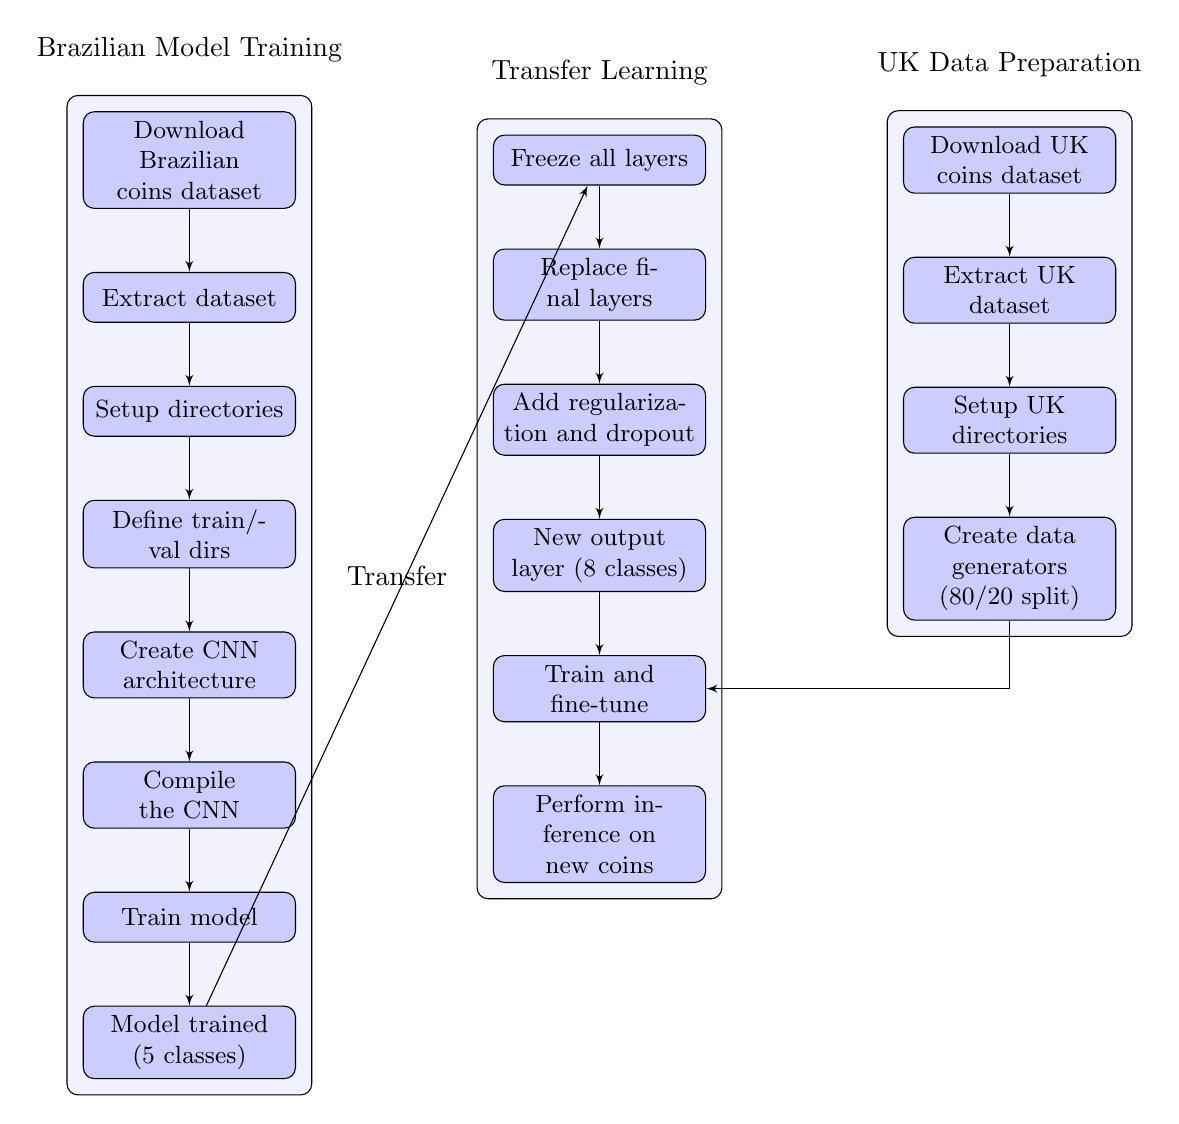
\begin{tikzpicture}[node distance=0.8cm and 1.5cm, auto]
    % Define a smaller block style
    \tikzset{
      block/.style = {rectangle, draw, fill=blue!20, 
                      text width=7em, text centered, rounded corners, minimum height=1.8em, font=\small},
    }
    
    % Brazilian model training - Column 1
    \node [block] (brazildata) {Download Brazilian coins dataset};
    \node [block, below=of brazildata] (extract) {Extract dataset};
    \node [block, below=of extract] (setup) {Setup directories};
    \node [block, below=of setup] (define) {Define train/val dirs};
    \node [block, below=of define] (create) {Create CNN architecture};
    \node [block, below=of create] (compile) {Compile the CNN};
    \node [block, below=of compile] (train) {Train model};
    \node [block, below=of train] (trained) {Model trained (5 classes)};
    
    % Transfer learning - Column 2 (Middle)
    \node [block, right=2.5cm of brazildata] (freeze) {Freeze all layers};
    \node [block, below=of freeze] (replace) {Replace final layers};
    \node [block, below=of replace] (add) {Add regularization and dropout};
    \node [block, below=of add] (output) {New output layer (8 classes)};
    \node [block, below=of output] (finaltrain) {Train and fine-tune};
    \node [block, below=of finaltrain] (inference) {Perform inference on new coins};
    
    % UK data preparation - Column 3 (Right)
    \node [block, right=2.5cm of freeze] (ukdata) {Download UK coins dataset};
    \node [block, below=of ukdata] (ukextract) {Extract UK dataset};
    \node [block, below=of ukextract] (uksetup) {Setup UK directories};
    \node [block, below=of uksetup] (ukgen) {Create data generators (80/20 split)};
    
    % Connect all nodes with arrows
    \path [line] (brazildata) -- (extract);
    \path [line] (extract) -- (setup);
    \path [line] (setup) -- (define);
    \path [line] (define) -- (create);
    \path [line] (create) -- (compile);
    \path [line] (compile) -- (train);
    \path [line] (train) -- (trained);
    
    \path [line] (ukdata) -- (ukextract);
    \path [line] (ukextract) -- (uksetup);
    \path [line] (uksetup) -- (ukgen);
    
    % Connect the columns
    \path [line] (trained) -- node[midway, above] {Transfer} (freeze);
    \path [line] (ukgen) |- (finaltrain);
    
    % Connect middle column
    \path [line] (freeze) -- (replace);
    \path [line] (replace) -- (add);
    \path [line] (add) -- (output);
    \path [line] (output) -- (finaltrain);
    \path [line] (finaltrain) -- (inference);
    
    % Group boxes to show different stages with smaller padding
    \begin{pgfonlayer}{background}
        \node[group={[yshift=0.3cm]above:Brazilian Model Training}, fit={(brazildata) (extract) (setup) (define) (create) (compile) (train) (trained)}, inner sep=0.2cm] {};
        \node[group={[yshift=0.3cm]above:UK Data Preparation}, fit={(ukdata) (ukextract) (uksetup) (ukgen)}, inner sep=0.2cm] {};
        \node[group={[yshift=0.3cm]above:Transfer Learning}, fit={(freeze) (replace) (add) (output) (finaltrain) (inference)}, inner sep=0.2cm] {};
    \end{pgfonlayer}
\end{tikzpicture}
}
% \caption{CNN Transfer Learning Flowchart: Brazilian to UK Coins}
% \label{fig:cnn-flowchart}
% \end{figure}
%     }
%     \caption{System Design Overview Flowchart}
%     \label{fig:decriptiveLabel6} % descriptive to call in text with \ref{fig:decriptiveLabel}
% \end{figure}

% \subsection{Functional Requirements}
% % Your content here

% \subsection{Design Approach}
% % Your content here

% \subsection{System Architecture}
% As shown in Figure~\ref{fig:decriptiveLabel6} the system architecture consists of various components.

% \begin{lstlisting}[style=cstyle, caption=System Architecture Code Example, label=lst:SystemArchitecture5]
% # Your code here
% \end{lstlisting}

% \begin{figure}[htbp] %h-ere t-op b-ottom p-page (separte) -good to allow all htbp to give the compiler more options
%     \centering
%     \includegraphics[width=0.6\textwidth]{figures/results/system_architecture.jpg}
%     \caption{System Architecture Diagram}
%     \label{fig:system-architecture21}
% \end{figure}
% % SystemPerformanceAnalysis.tex
\section{System Performance Analysis}

\subsection{Operational Constraints Identified}
% Your content here

\subsection{Environmental Factors Impact}
% Your content here



\subsection{System Stability and Repeatability}
% Your content here



\subsection{Recommendations for Improvement}
% Your content here



% Example figure jpg
%
% \begin{figure}[htb]
%     \centering
%     \includegraphics[width=1\textwidth]{figures/results/system_architecture.jpg}
%     \caption{Overall System Performance Analysis}
%     \label{fig:systemPerformance}
% \end{figure}

% Example listing (such as text output from console)
% \begin{figure}[H]
%     \begin{lstlisting}[style=cstyle]
%     // Environmental test results
%     // Temperature, ambient light, and vibration effects
%     \end{lstlisting}
%     \caption{Environmental Testing Results}
%     \label{lst:EnvironmentalTests1}
%     \end{figure}
% PrototypeComparison.tex
\section{Comparative Analysis}

To assess the accuracy of the developed simulation model, results from a full simulation run were compared against experimental data collected using the same sensor topology and an equivalent arc motion sequence.

Figure~\ref{fig:Model and Physical Results Comparison} presents a side-by-side comparison:
\begin{itemize}
    \item \textbf{Left:} Simulated illumination per sensor, expressed as the percentage of total emitted rays that intersected with each sensor area, plotted against the arc rotation angle.
    \item \textbf{Right:} Experimentally measured voltages from each physical sensor during the emitter's arc sweep. Signals have been filtered to reduce noise and highlight the response envelope.
\end{itemize}
\subsection*{Key Observations}
\begin{enumerate}
    \item \textbf{Overall Response Pattern:} Both plots show a clear progression of peak response across the sensor array. Sensor A2 activates first, followed by A1, A0, and then A3, which is consistent with the expected sequence during the rotation.
    
    \item \textbf{Peak Alignment:} The positions of the peak responses in the simulated and experimental plots align closely, suggesting that the source plane's movement and orientation in the simulation accurately reflects the RED testbench's real process.

\end{enumerate}
 \begin{landscape}
    \begin{figure}[htbp] %h-ere t-op b-ottom p-page (separte) -good to allow all htbp to give the compiler more options
        \centering
        \includegraphics[width=1.4\textwidth]{chapters/results/images/Comparison_plot.png} % change {path}
        \caption{Model and Physical Results Comparison}       % change {caption}
        \label{fig:Model and Physical Results Comparison}            % change label - used for reference in text
    \end{figure}
 \end{landscape}

The simulation and hardware behave in the same way, sensors are gradually illuminated and fade out as expected. The simulation appears to be handling the geometry correctly, and the physical sensor design works as intended.


\subsection*{Interpretation}
This result provides strong validation for:
\begin{itemize}
    \item The geometric modelling of planes, areas, and ray emission in the simulation framework.
    \item The arc rotation logic, particularly the ``rigid arc'' strategy where the plane consistently faces the origin.
    \item The accuracy of the designed sensor layout and aperture configuration.
\end{itemize}


% Example figure jpg
%
% \begin{figure}[htb]
%     \centering
%     \includegraphics[width=1\textwidth]{figures/results/system_architecture.jpg}
%     \caption{Overall System Performance Analysis}
%     \label{fig:systemPerformance}
% \end{figure}

% Example listing (such as text output from console)
% \begin{figure}[H]
%     \begin{lstlisting}[style=cstyle]
%     // Environmental test results
%     // Temperature, ambient light, and vibration effects
%     \end{lstlisting}
%     \caption{Environmental Testing Results}
%     \label{lst:EnvironmentalTests1}
%     \end{figure}
% SystemLimitationsAndConsiderations.tex
\section{System Limitations And Considerations}
This section discusses the limitations and future work.
\subsection{\acf{RED} testbench limitations and impact}
The Renewable Energy Demonstrator (RED) device borrowed from the EPS team \cite{RefWorks:shopov2022renewable} proved to be valuable as a testbench for our project, but several limitations affected our ability to gather comprehensive data for accurate sun vector determination.
\subsubsection{Servo Motor Limitations}
There were at least two issues with the Servo Motors which reduced our ability to gether data:
\begin{itemize}
    \item Inablity to reach the target angles requested in code without phisical intervention, presumably due to insufficient torque or gearing issues.
    \item Control deadband did not allow us to gather a large enough sample (small-angle adjustment) to create a \ac{LUT} that would allow the prediction of light position by extrapolation.
\end{itemize}

When attempting to move from 0\textdegree{} to 90\textdegree{}, for example, the servomotors would often stall, requiring manual assistance to ``help'' the arch reach the desired position. This introduced inconsistency in our testing methodology and required manual adjustment using protractors.

\subsubsection{Signal Interference Issues}

The \ac{RED}'s Power Supply interference make the signal very noisy. However due to the nature of the high frequency noise and low frequency signal, it meant that it was relativly easy to filter using the scipy.signal library \cite{RefWorks:butter}.

\subsection{Aperture placement accuracy}
% Your content here

% \subsection{}
% Your content here

% \subsection{}


% Example figure jpg
%
% \begin{figure}[htb]
%     \centering
%     \includegraphics[width=1\textwidth]{figures/results/system_architecture.jpg}
%     \caption{Overall System Performance Analysis}
%     \label{fig:systemPerformance}
% \end{figure}

% Example listing (such as text output from console)
% \begin{figure}[H]
%     \begin{lstlisting}[style=cstyle]
%     // Environmental test results
%     // Temperature, ambient light, and vibration effects
%     \end{lstlisting}
%     \caption{Environmental Testing Results}
%     \label{lst:EnvironmentalTests1}
%     \end{figure}



% Example LATEX flowchart
% Include a flowchart
% \begin{figure}[H]
%     \centering
%     \scalebox{0.8}{ % Scale to 80% of original size
%         % try generating flowcharts as svg in Claude 
% and edit with inkscape instead of this.
% but claude did generate this one so might 
% be useful too but you can't easily make
% small repairs in inkscape


% CNN Transfer Learning Flowchart - Compact Multi-Column Layout
% \begin{figure}[htbp]

\centering
\resizebox{\textwidth}{!}{ % Scale to fit width while maintaining aspect ratio
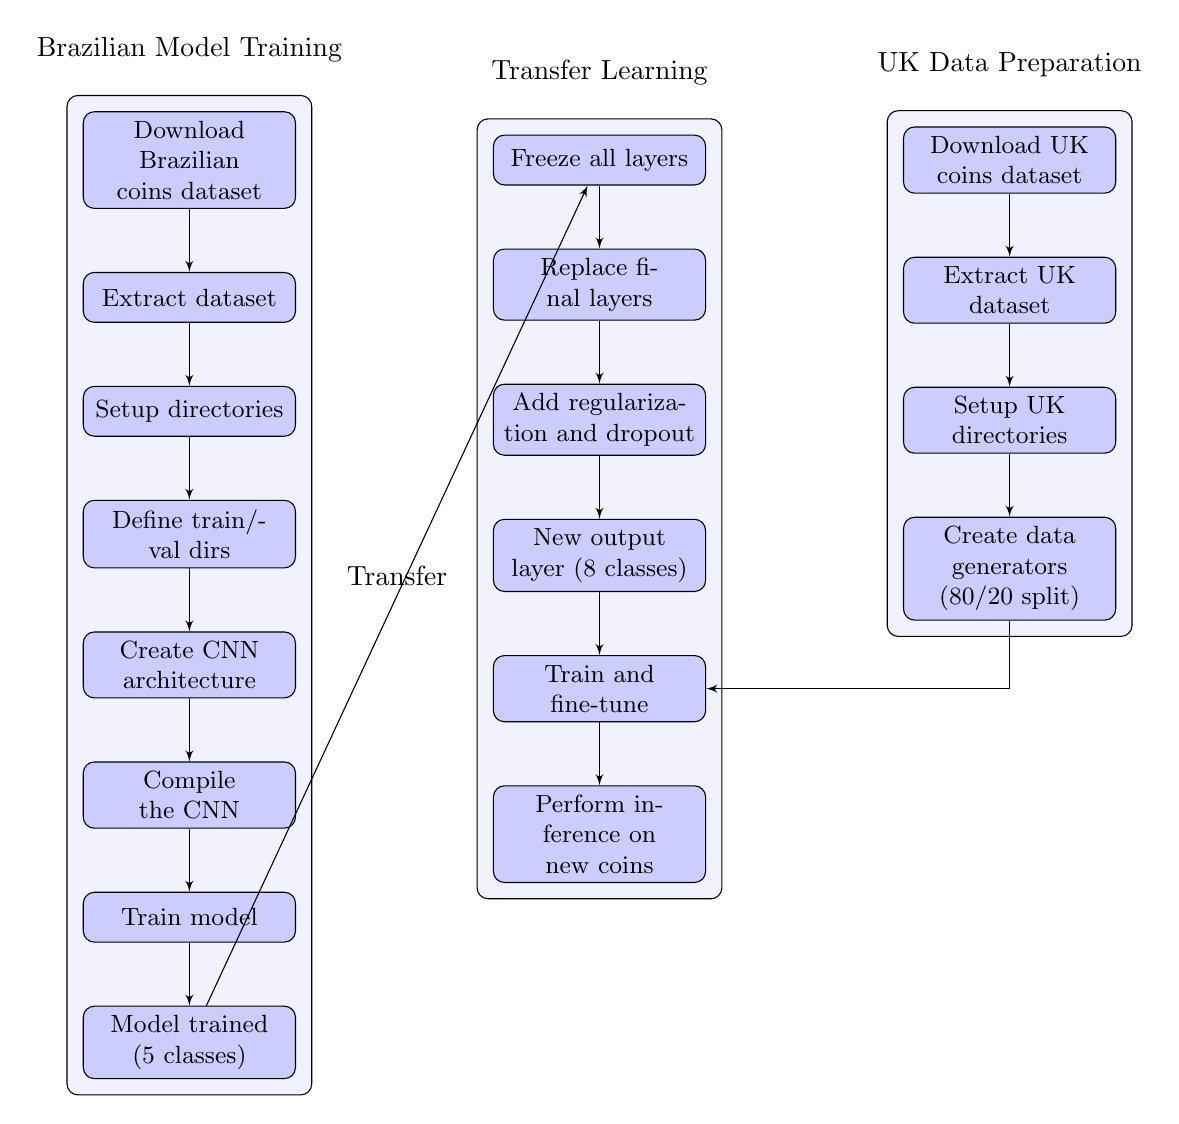
\begin{tikzpicture}[node distance=0.8cm and 1.5cm, auto]
    % Define a smaller block style
    \tikzset{
      block/.style = {rectangle, draw, fill=blue!20, 
                      text width=7em, text centered, rounded corners, minimum height=1.8em, font=\small},
    }
    
    % Brazilian model training - Column 1
    \node [block] (brazildata) {Download Brazilian coins dataset};
    \node [block, below=of brazildata] (extract) {Extract dataset};
    \node [block, below=of extract] (setup) {Setup directories};
    \node [block, below=of setup] (define) {Define train/val dirs};
    \node [block, below=of define] (create) {Create CNN architecture};
    \node [block, below=of create] (compile) {Compile the CNN};
    \node [block, below=of compile] (train) {Train model};
    \node [block, below=of train] (trained) {Model trained (5 classes)};
    
    % Transfer learning - Column 2 (Middle)
    \node [block, right=2.5cm of brazildata] (freeze) {Freeze all layers};
    \node [block, below=of freeze] (replace) {Replace final layers};
    \node [block, below=of replace] (add) {Add regularization and dropout};
    \node [block, below=of add] (output) {New output layer (8 classes)};
    \node [block, below=of output] (finaltrain) {Train and fine-tune};
    \node [block, below=of finaltrain] (inference) {Perform inference on new coins};
    
    % UK data preparation - Column 3 (Right)
    \node [block, right=2.5cm of freeze] (ukdata) {Download UK coins dataset};
    \node [block, below=of ukdata] (ukextract) {Extract UK dataset};
    \node [block, below=of ukextract] (uksetup) {Setup UK directories};
    \node [block, below=of uksetup] (ukgen) {Create data generators (80/20 split)};
    
    % Connect all nodes with arrows
    \path [line] (brazildata) -- (extract);
    \path [line] (extract) -- (setup);
    \path [line] (setup) -- (define);
    \path [line] (define) -- (create);
    \path [line] (create) -- (compile);
    \path [line] (compile) -- (train);
    \path [line] (train) -- (trained);
    
    \path [line] (ukdata) -- (ukextract);
    \path [line] (ukextract) -- (uksetup);
    \path [line] (uksetup) -- (ukgen);
    
    % Connect the columns
    \path [line] (trained) -- node[midway, above] {Transfer} (freeze);
    \path [line] (ukgen) |- (finaltrain);
    
    % Connect middle column
    \path [line] (freeze) -- (replace);
    \path [line] (replace) -- (add);
    \path [line] (add) -- (output);
    \path [line] (output) -- (finaltrain);
    \path [line] (finaltrain) -- (inference);
    
    % Group boxes to show different stages with smaller padding
    \begin{pgfonlayer}{background}
        \node[group={[yshift=0.3cm]above:Brazilian Model Training}, fit={(brazildata) (extract) (setup) (define) (create) (compile) (train) (trained)}, inner sep=0.2cm] {};
        \node[group={[yshift=0.3cm]above:UK Data Preparation}, fit={(ukdata) (ukextract) (uksetup) (ukgen)}, inner sep=0.2cm] {};
        \node[group={[yshift=0.3cm]above:Transfer Learning}, fit={(freeze) (replace) (add) (output) (finaltrain) (inference)}, inner sep=0.2cm] {};
    \end{pgfonlayer}
\end{tikzpicture}
}
% \caption{CNN Transfer Learning Flowchart: Brazilian to UK Coins}
% \label{fig:cnn-flowchart}
% \end{figure}
%     }
%     \caption{System Design Overview Flowchart}
%     \label{fig:decriptiveLabel4} % descriptive to call in text with \ref{fig:decriptiveLabel}
% \end{figure}
% Conclusions.tex
\chapter{Conclusions}

This project has successfully met its objective of developing a cost-effective and reliable analogue sun sensor system suitable for attitude determination in Low Earth Orbit (LEO) nanosatellite missions. Through the integration of hardware prototyping and software simulation, a robust methodology was established to evaluate the viability of photodiode-based sun sensing solutions.

A functional photodiode array was constructed, accompanied by a custom-designed signal conditioning circuit incorporating a transimpedance amplifier and post-amplification low-pass filtering. The system output was digitised using a Arduino-based data acquisition system, with post-processing conducted via Python to apply digital filtering and interpret results.

The software model, implemented in Python, facilitated accurate simulation of ray-plane interactions using geometric approximation. It enabled flexible configuration of sensor and aperture topologies, and supported visual and quantitative analysis of illumination results across a range of incident angles and positions. Comparative analysis between experimental and simulated data demonstrated strong correlation, validating the fidelity of the model and the underlying assumptions.

While the Renewable Energy Demonstrator (RED) testbench introduced some mechanical limitations, such as inconsistent servo performance and control noise, these were effectively mitigated through calibration, manual adjustments, and signal filtering techniques.

Ultimately, this project delivers a validated hybrid sun sensing system — combining practical prototyping with a software model.
% Your introduction content here
  
\chapter{Future Work}
%Mention: methods to avoid detecting sun reflections off the moon and earth (such as light intensity or light source width if possible).

%Unfortunately, there was no other easily available method of fabricating the apertures, such as having the apertures printed on glass with a fully opaque ink. Another method considered and attempted was to 3D print the apertures, but this would have resulted in the apertures having a thickness that would have changed the way the light enters, depending on the angle of the light.

\paragraph{Enhanced Aperture Design and Manufacturing}

The current prototype utilized manually placed apertures, resulting in alignment inconsistencies that affected measurement accuracy. 
Future iterations should explore precision manufacturing techniques such as photolithography or laser etching to create apertures with consistent placement and sharper edges. 
Additionally, testing alternative aperture geometries could optimize the sensor's field of view and accuracy across different incident angles.

\paragraph{Advanced Calibration Techniques}

Development of a comprehensive Look-Up Table (LUT) and interpolation algorithm would enable actual light position leading to attitude determination. 
Future work should include deploying the sensor on a high-precision platform to map responses across the entire field of view, generating a detailed calibration map.

\paragraph{Enviromnetla Qualification and Testing}

While thermal simulations suggested the viability of the design in space conditions, physical testing in thermal vacuum chambers would validate the sensor's performance under actual space-like conditions. 
Radiation testing would also be necessary to assess component degradation over an extended mission lifetime.

\paragraph{Discrimination capabilities}

Methods to avoid detecting sun reflections from the Earth, Moon, or spacecraft components should be investigated. 
Possibilities include implementing intensity thresholds, spectral filtering, or temporal signature analysis to distinguish direct solar illumination from reflected sources.


% Bibliography 
\bibliographystyle{IEEEtran}
\addcontentsline{toc}{chapter}{Bibliography}
\bibliography{bibliography/references}


% % Appendix
% \chapter*{Appendix}
% \addcontentsline{toc}{chapter}{Appendix}
% % Appendix content here
% \section{Full Code}
% %\lstinputlisting[language=Matlab]{matlab_code.m}

\end{document}